 % PRB regular article source -- channel-projected surgical revision
\documentclass[%
  aps,prb,reprint,amsmath,amssymb,superscriptaddress,longbibliography,floatfix
]{revtex4-2}

\usepackage{graphicx}
\usepackage{dcolumn}
\usepackage{bm}
\usepackage{physics}
\usepackage{hyperref}
\hypersetup{hidelinks}
\usepackage{xcolor}
\usepackage{booktabs}
\usepackage{enumitem}

\newcommand{\PT}{\mathcal{PT}}
\newcommand{\Hss}{H_{\rm ss}}
\newcommand{\Htilde}{\tilde{H}}
\newcommand{\teps}{\tilde{\epsilon}_{\xi}}
\newcommand{\keff}{\kappa_{\rm imp}}
\newcommand{\seff}{s_{\rm eff}}
\newcommand{\Eep}{E_{\rm EP}}
\newcommand{\Gless}{G^{<}}
\newcommand{\Gret}{G^{R}}
\newcommand{\Gadv}{G^{A}}
\newcommand{\tb}{\tilde{\beta}}          % gauge-invariant SBMF scale
\newcommand{\gb}{\beta_0}               % signed frozen drive-control amplitude
\newcommand{\gm}{\gamma}                % flip in frozen BA
\newcommand{\Gpt}{\Gamma_{\mathrm{PT}}}   % projected gain/loss channel
\newcommand{\dSig}{\delta_{\Sigma}}          % real one-body self-energy shift
\newcommand{\Deff}{\Delta_{\rm eff}}     % projected coherent splitting/flip
\newcommand{\Dzero}{\Delta_0}              % static coherent splitting in generic projection
\newcommand{\Dcoh}{\Delta_{\rm coh}}          % Kramers--Kronig coherent detuning
\newcommand{\Veff}{V_{\rm eff}}           % projected impurity-bath hybridization
\newcommand{\cGm}{c_{\Gamma}}
\newcommand{\cDl}{c_{\Delta}}
\newcommand{\cV}{c_V}
\newcommand{\mur}{\mu}                   % BA auxiliary rapidity

\begin{document}

\title{Emergent $\PT$ Symmetry and Exceptional Points
       in a Driven Dirac Impurity}

\author{Vinayak M.~Kulkarni}
\email{vmkphysimath@gmail.com}
\affiliation{Theoretical Sciences Unit,
  Jawaharlal Nehru Centre for Advanced Scientific Research,
  Bangalore 560064, India}

\date{\today}

\begin{abstract}
Periodic driving of correlated impurities can generate nonequilibrium steady
states, but the microscopic origin of passive non-Hermitian structures in such
systems is often obscured.  We show that a driven, inversion-asymmetric Dirac
impurity can realize a passive $\PT$-symmetric projected retarded kernel without
adding gain or loss to the microscopic Hamiltonian.  The construction proceeds
in two steps: off-shell auxiliary angular harmonics generate a real spin-odd
coherent shift, and embedding this shifted channel in an energy-dependent Dirac
bath converts it into a relative spin-dependent decay rate.  After subtracting
common bath damping, the co-decaying impurity kernel contains the passive
$\PT$ core $\Delta_{\rm eff}\sigma_x+i\Gamma_{\rm PT}\sigma_z$,
while the Kramers--Kronig partner $\Delta_{\rm coh}\sigma_z$ provides a causal
detuning floor that bounds the approach to exact coalescence.  We solve the
interacting impurity at the slave-boson mean-field level using the
gauge-invariant projected hybridization $\tilde\beta=|\beta_0||b_c|$ and the
physical bath-FDR spectrum.  Analytic Schrieffer--Wolff and frozen
Bethe-Ansatz-kernel estimates give the near-EP screening-scale enhancement;
independently, the SBMF spectra show positive spectral-weight transfer into
the shifted Friedel-type spectral resonance (FSR) associated with the Kondo feature in the same drive window.  The SBMF weight
transfer is not used as a definition of a thermodynamic Kondo temperature, and
FWHM-like linewidths are assigned only where the positive resonance is locally
resolved.  The result is a self-contained projected-kernel description of how
impurity-localized passive-\(\PT\) nonnormality can enhance low-energy
screening diagnostics while preserving causality of the underlying Hermitian
system.
\end{abstract}

\maketitle

% ============================================================
\section{Introduction}
\label{sec:intro}
% ============================================================

Driven quantum systems provide a versatile route to steady states
and dynamical phases that have no equilibrium analogs.
When coherent drive, dissipation, and strong correlations coexist,
the resulting many-body dynamics can generate fixed points that
reflect both microscopic symmetry and emergent non-Hermitian
structure.
Recent work has shown that minimizing a driven bosonic field within
a Keldysh mean-field framework can reproduce renormalization-group
(RG)-like fixed points~\cite{kamenev2023field,popruzhenko2014keldysh,maghrebi2016nonequilibrium},
pointing to a deeper connection between nonequilibrium stability
and non-Hermitian criticality~\cite{kulkscipo,Claeys2022RGdissipative}.

Exceptional points (EPs) are non-Hermitian degeneracies where
eigenvalues and eigenvectors coalesce, playing a central role in
such settings.
They reshape spectral topology and enable non-reciprocal transport,
sensing enhancement, and dynamical control.
EPs have been linked to the non-Hermitian skin
effect~\cite{PhysRevLett.121.203001}, higher-order
degeneracies~\cite{higherorder,PhysRevLett.126.110404},
and ultrafast projective protocols in both quantum and classical
experiments~\cite{wan2023evidence,mentink2015ultrafast}.
Their influence extends beyond spectra: non-Hermitian topology
underpins phenomena in nonlinear
photonics~\cite{xia2021nonlinear,smirnova2020nonlinear},
topological acoustics~\cite{xue2022topological},
engineered metamaterials~\cite{RevModPhys.96.015002};
coherent light--matter
coupling and engineered dissipation can stabilize correlated states
such as topological Kondo phases~\cite{hu2025ceco2p2}, and
nonlinearities can generate instabilities captured by dynamical
mean-field theory~\cite{aoki2014nonequilibrium,PhysRevX.7.031013}.

Impurity systems are particularly sensitive to anisotropy and
dissipation.
Boundary-induced openness can mimic potential
scattering~\cite{kattel2024kondo,kattel2024spin,kattel2024dissipation},
while nonlinear perturbations modify inelastic processes and impurity
coherence.
Non-Hermitian phase transitions have recently been observed in
condensed-matter
experiments~\cite{li2024discoverynonhermitianphasetransition},
and nonlinear optical platforms provide precise control of
non-Hermitian
topology~\cite{dai2024non,PhysRevLett.132.156901,khanikaev2024topological}.
In correlated impurity models, non-Hermitian features manifest
through sign reversals in RG flows and causality violations in both
interacting and non-interacting
settings~\cite{PhysRevB.111.125157,han2023complex,
PhysRevB.111.045124,kulkscipo}.
Non-Hermitian Kondo physics has been explored via numerical
renormalization group, cold-atom platforms, and Floquet-engineered
conduction bands~\cite{burke2025non,19td-1k9s,
PhysRevLett.121.203001,PhysRevB.108.155120,SBkeld}.
Integrability of the Kondo model with time-dependent couplings
has been established via quantum Knizhnik--Zamolodchikov
equations~\cite{pasnoori2025tdkondo}, and a $\PT$-protected
Kondo effect has been observed in
CeCo$_2$P$_2$~\cite{hu2025ceco2p2}.
Benchmark studies of the two-dimensional Hubbard model have
established the regime of validity of large-$N$ slave-boson and
mean-field treatments of correlated
electrons~\cite{simons2015hubbard}, directly motivating the
approach employed in Sec.~\ref{sec:mf}.

Here we show that a driven impurity embedded in a Dirac-like bath
naturally develops a passive non-Hermitian kernel once higher angular
harmonics and the energy-dependent Dirac bath are treated together.
The off-shell auxiliary harmonics generate a real spin-odd coherent
shift.  The retarded Dirac bath, whose width depends on energy and
spin-orbit structure, converts this shift into a spin-dependent decay
rate.  After subtracting the common bath damping, the remaining
co-decaying kernel contains a dynamically induced passive
$\PT$-symmetric core, together with a Kramers--Kronig-related coherent
detuning that bounds the approach to exact coalescence.
We demonstrate that the resulting finite-drive near-EP structure
persists under thermal equilibration and under self-consistent
minimization---despite arising without any explicit non-Hermitian term
in the microscopic Hamiltonian.
\emph{In contrast to earlier studies where non-Hermiticity is
imposed phenomenologically or emerges through renormalization-group
flow~\cite{PhysRevLett.121.203001,han2023complex,
PhysRevB.111.045124}, we demonstrate a complementary microscopic
route in which a strictly Hermitian, periodically driven Dirac impurity
produces a passive non-Hermitian relative kernel after coarse graining
and removal of the common decay.}
Dirac baths provide a natural setting because spin--momentum
locking, angular-momentum selection rules, and an energy-dependent
spectral width make the passive $\PT$ channel symmetry constrained.

The paper is organized as follows.
Section~\ref{sec:model} defines the full Hermitian Hamiltonian.
Section~\ref{sec:coarse} performs the bilinear Gaussian coarse graining
and establishes the emergent $\PT$ symmetry.
Section~\ref{sec:Hss} derives the steady-state Hamiltonian and
the Hadamard rotation that makes hybridization diagonal.
Section~\ref{sec:mf} presents the slave-boson mean field and
the resulting shifted resonance condition.
Sections~\ref{sec:spectra}--\ref{sec:FDR} show spectral properties,
phase-selective EP diagnostics, and the fluctuation--dissipation
relation (FDR).  Section~\ref{sec:dynamics} discusses real-time dynamics
in the passive co-decaying frame.  Section~\ref{sec:BA} presents the
biorthogonal Bethe Ansatz (BA) for the frozen effective model.
Section~\ref{sec:kondo} discusses near-EP low-energy scale estimates within slave-boson mean-field (SBMF) theory.
Section~\ref{sec:conc} concludes.

% ============================================================
\section{Model and Hamiltonian}
\label{sec:model}
% ============================================================

The full Hermitian Hamiltonian is
$H=H_{\rm bath}+H_{\rm imp}+H_{\rm imp\text{-}bath}+H_O+H_{\rm hyb}[\phi(t)]$.
Each term has a distinct physical role.
$H_{\rm bath}$ describes the two-dimensional Dirac conduction band
with spin-orbit coupling.
$H_{\rm imp}$ is the correlated Anderson impurity.
$H_{\rm imp\text{-}bath}$ is the bare hybridization between the
impurity and the $m=0$ bath channel.
$H_O$ represents auxiliary angular-momentum modes generated by
the trigonal crystal anisotropy.
$H_{\rm hyb}$ couples the physical bath to the angular harmonics
and is modulated by the periodic drive.
We define all symbols at first use below.  To prevent notation clashes,
we reserve $t_{\rm av}=(t+t')/2$ and $\tau=t-t'$ for the Wigner center and
relative times, respectively, and use $T_{\rm b}$ only for the reservoir
temperature.  The chiral bath index is $\eta=\pm$, whereas
$\zeta_\sigma=+1$ ($-1$) for $\sigma=\uparrow$ ($\downarrow$).
The SOC strength is $\lambda$; $\beta_0$ is the signed frozen drive-control
amplitude; and $\tilde\beta=|\beta_0||b_c|$ is its nonnegative
SBMF-renormalized projection.  The radial momentum cutoff $k_{\rm max}$ and
the ultraviolet energy cutoff $D_{\rm uv}$ are conceptually distinct; in the
dimensionless plots both are set numerically to $\pi/4$ as a convention.
We denote the analytic bare-block EP by
$\beta_{0,{\rm bare}}^{\rm EP}=\gamma=0.50$ and the full projected
numerical value by $\beta_{0,{\rm proj}}^{\rm EP}=0.4975$.

\subsection{Bath}

We consider a two-dimensional (2D) host crystal with trigonal ($C_3$)
anisotropy.
The conduction electrons form a Dirac bath with spin-orbit coupling (SOC):
\begin{equation}
H_{\rm bath}
= \sum_{k,\sigma}\epsilon_k\,c^\dagger_{k\sigma}c_{k\sigma}
+ \lambda\sum_k k
  \bigl(c^\dagger_{k\uparrow}c_{k\downarrow}+\mathrm{h.c.}\bigr),
\label{eq:Hbath}
\end{equation}
where $c^\dagger_{k\sigma}$ creates a bath electron with radial
momentum $k$ (in units of inverse lattice constant) and spin
$\sigma\in\{\uparrow,\downarrow\}$;
$\epsilon_k=\alpha_{\rm b}k^2$ ($\alpha_{\rm b}>0$), with radial cutoff
$0\le k\le k_{\rm max}=\pi/4$; and $\lambda>0$ is the spin-orbit
coupling.  The separate energy cutoff $D_{\rm uv}$ enters only logarithmic
and scaling formulas below.
The chiral rotation
$c_{k\pm}=(c_{k\uparrow}\pm c_{k\downarrow})/\sqrt{2}$
diagonalizes $H_{\rm bath}$ exactly, yielding SOC-split chiral
dispersions $\varepsilon_{k\pm}=\alpha_{\rm b}k^2\pm\lambda k$ with
$\varepsilon_{k+}\neq\varepsilon_{k-}$ for all $k\neq0$.
Near the Dirac point the bath density of states is
$\rho_{\rm bath}(\omega)\sim|\omega|/\lambda^2$~\cite{kulkscipo},
which is the origin of the pseudogap structure explored in
Secs.~\ref{sec:mf}--\ref{sec:spectra}.

\subsection{Impurity}

The correlated impurity is described by the Anderson Hamiltonian:
\begin{equation}
H_{\rm imp}
=\sum_\sigma\epsilon_\xi\,d^\dagger_\sigma d_\sigma
+ U\,n_\uparrow n_\downarrow,
\label{eq:Himp}
\end{equation}
where $d^\dagger_\sigma$ creates an impurity electron with spin
$\sigma$, $n_\sigma=d^\dagger_\sigma d_\sigma$ is the occupation,
$\epsilon_\xi$ is the bare impurity level before the projected
bath-induced detuning is included, and $U>0$ is the on-site Coulomb
repulsion.

\subsection{Impurity--Bath Hybridization}

The impurity couples directly to the $m=0$ (s-wave) bath channel via
\begin{equation}
H_{\rm imp\text{-}bath}
=\sum_{k,\sigma}
\left(W_k\,c^\dagger_{k,0,\sigma} d_\sigma + \mathrm{h.c.}\right),
\label{eq:Hcd}
\end{equation}
where $W_k$ is the bare hybridization amplitude.
This term defines the physical coupling between the impurity and the
conduction bath before the angular-momentum harmonics are introduced.

In the presence of the driven angular-momentum sector
[Eqs.~(\ref{eq:HO})--(\ref{eq:Hhyb})], the $m=0$ bath propagator
becomes dressed by virtual processes involving the auxiliary modes
$m\neq0$: the auxiliary modes generate a retarded self-energy
$\Sigma_\sigma^{\rm bath}$ on the $m=0$ bath channel
(Sec.~\ref{sec:coarse}).
The impurity self-energy then arises from this dressed bath
propagator through Eq.~(\ref{eq:Hcd}):
it is the auxiliary dressing of the bath propagator, communicated
to the impurity via the bare coupling $W_k$, that produces the
effective non-Hermitian self-energy on the impurity sector.
This two-step mechanism---auxiliary modes dress the bath, bath
dresses the impurity---is made explicit in Sec.~\ref{sec:coarse}
and Supplemental Material.

\subsection{Auxiliary Angular-Momentum Modes}

The trigonal anisotropy $\beta_3(k)k^3\cos3\theta$ of the host crystal
(where $\beta_3(k)$ is the momentum-dependent trigonal crystal-field strength,
distinct from the hybridization amplitude $\gb$ introduced below;
and $\theta$ is the in-plane momentum angle) couples the
$m=0$ (s-wave) bath channel to higher angular-momentum harmonics
$m=\pm3,\pm6,\ldots$ via the $C_3$ selection rule $\Delta m=\pm3$.
These higher harmonics are represented by auxiliary fermions
$O_{k,m,\sigma}$ with angular momentum index $m\neq0$:
\begin{equation}
\begin{split}
    H_O=\sum_{k,m\neq0,\sigma}
\epsilon_O^{(m)}\,&O^\dagger_{k,m,\sigma}O_{k,m,\sigma}\\
&+\sum_{k,m,\sigma}\beta_3(k)k^3
O^\dagger_{k,m+3,\sigma}O_{k,m,\sigma}\\
&\quad+\mathrm{h.c.},
\label{eq:HO}
\end{split}
\end{equation}
where the mode energies satisfy $\epsilon_O^{(m)}=\epsilon_O^{(-m)}$
(inversion symmetry of the crystal).  The fields $O_{k,m,\sigma}$
should be understood as a Feshbach, or Loewdin-partitioned, representation
of remote higher-angular-harmonic crystal-field channels rather than as
an additional low-energy bath.  Their energies include the local orbital
or crystal-field splitting of these nonresonant harmonics relative to
the active $m=0$ Dirac channel.  In the low-energy limit
$\epsilon_O^{(m)}\gg D_{\rm uv}$, the auxiliary modes are therefore far off-shell
and can be integrated out exactly within the quadratic sector; their
main effect is a principal-value self-energy dressing the $m=0$ bath
propagator, which in turn induces a self-energy in the impurity sector
through the bare hybridization Eq.~(\ref{eq:Hcd})
(see Sec.~\ref{sec:coarse} and Supplemental Material).  If an
auxiliary harmonic approaches the conduction-band window, the same
formalism gives an ordinary on-shell bath damping contribution; this
spin-even damping is not identified with the passive relative $\PT$ channel.


\subsection{Periodic Drive and Hybridization}

The periodic drive couples the physical bath ($m=0$) to the remote
higher angular harmonics.  We write the Hermitian bath--auxiliary
hybridization as
\begin{equation}
\begin{split}
H_{\rm hyb}[\phi(t)]
=&\sum_{k,\theta,\sigma,m\neq0}
\bigl[
V_m(k)e^{i3m\theta}e^{i\zeta_\sigma\phi(t)} \\
&\hspace{1.2cm}\times
c^\dagger_{k,\theta,\sigma}O_{k,m,\sigma}
+\mathrm{h.c.}\bigr] .
\end{split}
\label{eq:Hhyb}
\end{equation}
Here $\zeta_\uparrow=+1$ and $\zeta_\downarrow=-1$ label the spin-helicity
channel selected by the spin-orbit-split Dirac bath, while
$\phi(t)=(\pi/4)\sin(\Omega t)$ is the slow drive phase.  In the passive
mechanism the frozen control is the instantaneous angular velocity
$\dot\phi(t_{\rm av})=(\pi\Omega/4)\cos(\Omega t_{\rm av})$; the numerical parameter
$\gb$ used below should be read as the corresponding effective
frozen-kernel amplitude, not as the value of the phase itself.  Hermiticity
fixes the second vertex to carry the complex-conjugate phase.  Therefore
the normal Gaussian contraction of a number-conserving auxiliary sector
contains phase differences, not phase sums.  This is important: the
off-shell auxiliary sector does not by itself generate anti-Hermitian
gain or loss.

Equivalently, the phase can be removed from Eq.~(\ref{eq:Hhyb}) by the
time-dependent unitary rotation
\begin{equation}
O_{k,m,\sigma}\rightarrow e^{-i\zeta_\sigma\phi(t)}O_{k,m,\sigma} .
\label{eq:aux_gauge_rotation}
\end{equation}
The vertices then become phase-free, while the auxiliary Hamiltonian
acquires the Berry term
\begin{equation}
\epsilon_O^{(m)}\rightarrow
\epsilon_O^{(m)}-\zeta_\sigma\dot\phi(t) .
\label{eq:aux_level_shift}
\end{equation}
Thus a gapped Hermitian auxiliary sector produces, in the adiabatic
low-energy projection, a real spin-odd coherent shift.  The passive
non-Hermitian component appears only in the second step, when this
shifted channel is embedded in the energy-dependent retarded Dirac
bath.
For the Gaussian projection the relevant adiabatic hierarchy is
$\Omega\ll\epsilon_O^{(m)}$; the separate Kondo steady-state
interpretation is restricted to the finite-drive window where the
extracted screening scale exceeds the drive frequency.  Because $H_O$ is
\emph{bilinear} in $O_{k,m,\sigma}$, the modes $m\neq0$ can be integrated
out at the Gaussian level without approximation within the quadratic
sector; the interaction $U$ enters only through the slave-boson mean field
on the impurity level (Sec.~\ref{sec:Hss}).

% ============================================================
\section{Coarse Graining and Emergent $\PT$ Symmetry}
\label{sec:coarse}
% ============================================================

This section isolates the bilinear coarse graining from the later
slave-boson mean-field treatment of the local interaction.  The raw
retarded self-energy generated by the auxiliary angular modes is, in
general, a complex retarded function; it is not assumed to be positive.
The $\PT$-active low-energy kernel is obtained by projecting the
spin-dependent impurity self-energy onto a spin-conjugate pair
$z,z^*$.  This formulation keeps the microscopic origin of the passive
relative gain--loss channel explicit while avoiding any assumption that the raw
retarded envelope is real, positive, or sign definite.


\subsection{Keldysh Path Integral and Angular-Mode Integration}

We work within the Keldysh formalism~\cite{kamenev2023field}, writing
the partition function as a coherent-state path integral on the closed
time contour.  The bath and auxiliary angular modes enter quadratically
and can be eliminated at the Gaussian level.  The local Coulomb
interaction on the impurity is not treated in this Gaussian step; it is
incorporated later through the slave-boson mean-field approximation in
Sec.~\ref{sec:mf}.

The Grassmann integration can be written explicitly.  For fixed
$(k,\theta,\sigma)$, collect the auxiliary fields into a vector
$O=(\ldots,O_{m},\ldots)^T$ and write the quadratic contour action as
\begin{equation}
\begin{split}
S_O+S_{cO}=&
\int_{\mathcal C} dt dt'\,\bar O(t) A_O(t,t')O(t') \\
&+\int_{\mathcal C} dt\,
\left[\bar c(t)V_\sigma(t)O(t)+
\bar O(t)V_\sigma^\dagger(t)c(t)\right].
\end{split}
\label{eq:grassmann_aux_action}
\end{equation}
The Gaussian identity for Grassmann variables gives
\begin{align}
\int \mathcal D[\bar O,O]e^{i(S_O+S_{cO})}
&\propto \det A_O\,e^{iS_{\rm infl}},
\label{eq:grassmann_identity}\\
S_{\rm infl}
&=-\int_{\mathcal C}dt dt'\,
\bar c(t)\,\Xi_\sigma(t,t')\,c(t'),
\label{eq:grassmann_influence_main}\\
\Xi_\sigma(t,t')
&=V_\sigma(t)g_O(t,t')V_\sigma^\dagger(t') .
\label{eq:Xi_aux_kernel}
\end{align}
Here $g_O=A_O^{-1}$ is the contour auxiliary propagator.  This is the
complete Gaussian step: because the auxiliary sector conserves particle
number, there is no anomalous $OO$ contraction.  Keeping both vertices of
Eq.~(\ref{eq:Hhyb}) explicit, the normal auxiliary contraction gives
\begin{align}
\Sigma_{\sigma}^{O,R}(t,t')
&=\sum_{m,m'\neq0}
 v_{m\sigma}(t)\,
 g_{mm'}^{O,R}(t,t')\,
 v^*_{m'\sigma}(t'),
\label{eq:normal_aux_contraction}\\
v_{m\sigma}(t)
&=V_m e^{i3m\theta}e^{i\zeta_\sigma\phi(t)} .
\label{eq:normal_aux_vertex}
\end{align}
For the diagonal terms, and also for any Hermitian off-shell auxiliary
matrix after summing conjugate paths, the phases enter as
$e^{i\zeta_\sigma[\phi(t)-\phi(t')]}$.  In Wigner coordinates this becomes
$1+O(\Omega/\epsilon_O)$ and gives a regular Hermitian
principal-value shift.  Equivalently, after the unitary rotation in
Eq.~(\ref{eq:aux_gauge_rotation}), the same result is obtained from the
spin-dependent level shift in Eq.~(\ref{eq:aux_level_shift}).

To leading order in the slow drive and in the off-shell expansion, the
auxiliary-dressed $m=0$ bath therefore has the form
\begin{equation}
\begin{split}
\Sigma_{\sigma}^{\rm bath,R}(\omega,t_{\rm av})
=&\,\Sigma_0^{\rm bath,R}(\omega)
+\zeta_\sigma\Delta_{\rm aux}(\omega,t_{\rm av}) \\
&+O\!\left[(\Omega/\epsilon_O)^2\right] .
\end{split}
\label{eq:aux_real_shift}
\end{equation}
Here $\Delta_{\rm aux}$ is real in the low-energy window.  Microscopically
one may write, schematically,
\begin{equation}
\begin{split}
\Delta_{\rm aux}(\omega,t_{\rm av})
=&-\dot\phi(t_{\rm av})\,\partial_{\epsilon_O}
\sum_{m\neq0}|V_m|^2 \\
&\times
\mathcal{P}\frac{1}{\omega-\epsilon_O^{(m)}} ,
\end{split}
\label{eq:Delta_aux}
\end{equation}
up to form-factor and angular-overlap coefficients.  If an auxiliary
pole enters the conduction window, the corresponding delta-function
part gives ordinary bath damping; it is not identified with the passive
$\PT$ channel.

The bare impurity--bath hybridization $W_k$ in
Eq.~(\ref{eq:Hcd}) remains time independent.  The drive reaches the
impurity through the dressed bath propagator.  In contour notation the
two Gaussian eliminations give
\begin{align}
G_{c,\sigma}^{-1}
&=g_c^{-1}-\Xi_\sigma,
\qquad
\Xi_\sigma=V_\sigma\circ g_O\circ V_\sigma^\dagger,
\label{eq:dressed_c_inverse}\\
\Sigma_{d,\sigma}
&=W^\dagger\circ G_{c,\sigma}\circ W,
\label{eq:impurity_selfenergy_dressed_bath}
\end{align}
where $\circ$ denotes contour convolution.  Thus the drive-dependent
virtual path is $d\to c\to O\to c\to d$; no direct time dependence of
$W_k$ is required.  The full Schur-complement derivation is given in the
Supplemental Material.

In the frozen off-shell window, write
$\Xi_\sigma^R=\Xi_0^R+\zeta_\sigma\delta\Xi^R$ with
$\delta\Xi^R\in\mathbb R$.  Expanding the dressed-bath resolvent gives the
general first-order correction
\begin{equation}
\delta\Sigma_d^R
=W^\dagger G_{c,0}^R\,\delta\Xi^R\,G_{c,0}^R W .
\label{eq:deltaSigma_exact}
\end{equation}
Although the auxiliary correction is real, the retarded continuum
propagators are complex, so the transmitted impurity correction has both
coherent and dissipative parts.  Defining
\begin{equation}
\Sigma_{d,0}^R(\omega)=\Lambda(\omega)-i\bar\Gamma(\omega),
\label{eq:Sigma0_Lambda_Gamma}
\end{equation}
we write
\begin{equation}
\Sigma^R_{d,\sigma}
=\Sigma_{d,0}^R+\zeta_\sigma\Delta_{\rm coh}
+i \zeta_\sigma\Gamma_{\rm PT}.
\label{eq:Delta_Gamma_PT}
\end{equation}
For the nearly rigid scalar shift used in the analytic estimates,
$\delta\Xi^R\simeq\Delta_{\rm aux}$ and the spin-even auxiliary
background varies slowly.  Then
\begin{equation}
\Sigma^R_{d,\sigma}(\omega,t_{\rm av})
\simeq
\Sigma_{d,0}^R(\omega-\zeta_\sigma\Delta_{\rm aux})
\simeq
\Sigma_{d,0}^R-\zeta_\sigma\Delta_{\rm aux}
\partial_\omega\Sigma_{d,0}^R,
\label{eq:Dirac_conversion}
\end{equation}
which gives
\begin{equation}
\Delta_{\rm coh}=-\Delta_{\rm aux}\partial_\omega\Lambda,
\qquad
\Gamma_{\rm PT}=\Delta_{\rm aux}\partial_\omega\bar\Gamma .
\label{eq:Delta_Gamma_defs}
\end{equation}
Equation~(\ref{eq:deltaSigma_exact}) is the general first-order result;
Eq.~(\ref{eq:Dirac_conversion}) is its rigid-shift limit.  All functions
are evaluated in the active low-energy window.
Equations~(\ref{eq:Dirac_conversion})--(\ref{eq:Delta_Gamma_defs}) show why the
Dirac bath is essential: for a flat wide band with
$\partial_\omega\bar\Gamma=0$, the same auxiliary shift would only
produce a coherent spin splitting, not a passive $\PT$ decay imbalance.
The SOC split bath also supplies the spin--momentum-locked helicity
channels.  In the chiral basis,
\begin{align}
\bar\Gamma_\eta(\omega)
&=\pi\sum_k |W_{k\eta}|^2
\delta\!\left(\omega-\varepsilon_{c,\eta}(k)\right),
\label{eq:helicity_width}\\
\varepsilon_{c,\eta}(k)&=\alpha_{\rm b}k^2+\eta\lambda k .
\label{eq:helicity_dispersion}
\end{align}
so the SOC parameter $\lambda$ controls the channel density of states,
the slope $\partial_\omega\bar\Gamma_\eta$, and the form factor entering
the projected EP diagnostics.  Without SOC-induced helicity structure
and energy-dependent Dirac spectral weight, the auxiliary shift remains a
coherent real field rather than a passive relative decay channel.


\subsection{Passive $\PT$ Core and Causal Detuning}
\label{sec:PT_all}

The projected impurity self-energy is decomposed into a common bath part,
a passive relative decay imbalance, and a Kramers--Kronig-related coherent
detuning:
\begin{equation}
\begin{split}
\Sigma_{\rm imp}^{R}(\omega,t_{\rm av})=&
\left[\Lambda(\omega)-i\bar\Gamma(\omega)\right]\mathbb{I} \\
&+\Dcoh(\omega,t_{\rm av})\sigma_z
+i\Gamma_{\rm PT}(\omega,t_{\rm av})\sigma_z .
\end{split}
\label{eq:passive_PT_selfenergy}
\end{equation}
The first line is a common Lamb shift and common decay.  It is retained in
the bath-controlled FDR, but it does not affect the relative EP structure.
The second line contains two spin-odd terms with different symmetry status:
$i\Gamma_{\rm PT}\sigma_z$ is the passive relative decay imbalance, while
$\Dcoh\sigma_z$ is a real coherent detuning generated by the same causal
retarded bath self-energy.

The SOC bath supplies the Hermitian spin-mixing channel.  In the original
spin basis, the local bath Green function has the matrix structure
\begin{equation}
\begin{split}
g_b^R(k,\omega)
&=\left[\omega^+-\epsilon_k-\lambda k\sigma_x\right]^{-1} \\
&=g_0(k,\omega)\mathbb{I}+g_x(k,\omega)\sigma_x,
\end{split}
\label{eq:soc_bath_matrix}
\end{equation}
with
\begin{equation}
g_x(k,\omega)=
\frac{\lambda k}
{(\omega^+-\epsilon_k)^2-\lambda^2 k^2} .
\label{eq:soc_bath_gx}
\end{equation}
The principal-value part of this SOC off-diagonal bath dressing gives a
real coherent spin-mixing coefficient,
\begin{equation}
\Deff(\omega)=
\sum_k |W_k|^2\, {\rm Re}\, g_x(k,\omega),
\label{eq:Delta_eff_soc_origin}
\end{equation}
renormalized in the interacting problem by the slave-boson saddle point.
The drive-induced shift cannot leak into this mixing channel at leading
order: expanding the dressed bath propagator to first order in the
spin-odd shift $\Delta_{\rm aux}\sigma_z$ gives
\begin{equation}
g_b^R\,\sigma_z\,g_b^R=\left(g_0^2-g_x^2\right)\sigma_z,
\label{eq:sigma_z_purity}
\end{equation}
because $\{\sigma_x,\sigma_z\}=0$, so the first-order correction is
purely $\sigma_z$ and $\Deff$ remains a static (drive-independent)
channel at this order, corresponding to the offset $\Dzero$ of
Eq.~(\ref{eq:projected_channels}); the isolated finite-drive EP of the
generic projection is therefore the microscopically natural case.
Thus, after subtracting the common damping, the general relative two-channel
kernel is
\begin{equation}
h_{\rm rel}=
\Deff\sigma_x+
\left(\Dcoh+i\Gamma_{\rm PT}\right)\sigma_z .
\label{eq:relative_detuned_kernel}
\end{equation}
The passive-$\PT$-symmetric core is obtained at the compensated detuning
point $\Dcoh=0$:
\begin{equation}
h_{\PT}=
\Deff\sigma_x+i\Gamma_{\rm PT}\sigma_z,
\qquad
\sigma_x h_{\PT}^*\sigma_x=h_{\PT} .
\label{eq:passive_PT_core}
\end{equation}
The real term $\Dcoh\sigma_z$ is not discarded.  It is $\PT$-odd under the
same operation and therefore acts as a causal detuning floor.  The pole
splitting of Eq.~(\ref{eq:relative_detuned_kernel}) is
\begin{equation}
s^2=
\Deff^2+
\left(\Dcoh+i\Gamma_{\rm PT}\right)^2 .
\label{eq:detuned_EP_splitting}
\end{equation}
For real $\Deff$, $\Dcoh$, and $\Gamma_{\rm PT}$, exact coalescence in the
passive sector requires
\begin{equation}
\Dcoh\Gamma_{\rm PT}=0,
\qquad
\Deff^2+\Dcoh^2-\Gamma_{\rm PT}^2=0 .
\label{eq:detuned_EP_conditions}
\end{equation}
Thus, for a nonzero relative decay imbalance, the exact passive EP occurs
at the compensated point $\Dcoh=0$ and $|\Deff|=|\Gamma_{\rm PT}|$.
Compensation is an operating-energy condition rather than a fine tuning:
$\Dcoh\propto\partial_\omega\Lambda$ changes sign and vanishes at a
finite energy of order $D_{\rm uv}/e$ for the linear Dirac width, where
$\partial_\omega\bar\Gamma$ remains finite, while near the Fermi level
the companion ratio is logarithmically enhanced,
$|\Dcoh/\Gamma_{\rm PT}|\simeq(2/\pi)\ln(D_{\rm uv}/|\omega|)$.  Away from the
compensated point, the Kramers--Kronig detuning prevents a literal pole
coalescence: minimizing $|s|$ over $\Deff$ at fixed $\Dcoh$ and
$\Gamma_{\rm PT}$ gives the causal floor
\begin{equation}
|s|_{\rm min}=\sqrt{2\,|\Dcoh|\,\Gamma_{\rm PT}}\,,
\label{eq:KK_floor}
\end{equation}
with the same square-root non-analyticity as the interaction floor
$\seff=[U\gb\sqrt{F(\lambda)}]^{1/2}$ of the Supplemental Material, where $F(\lambda)$ is the SOC-overlap form factor: causality and
interactions regularize the EP with the identical functional form.  The
figures should therefore be read as near-EP diagnostics of the
co-decaying projected kernel, consistent with the bounded
$Z_{\eta}^{\rm bio}$ and $s_{\min}$ regularization used in the
BA-kernel analysis.

This two-step structure is the microscopic origin of the kernel used in
the rest of the paper: off-shell auxiliary modes generate a real spin-odd
shift; the energy-dependent Dirac bath converts that shift into a
spin-dependent width; and the SOC bath provides the Hermitian spin-mixing
channel.  The numerical scans treat $\gb$ as a tunable frozen effective
kernel control parameter.  Microscopically,
\begin{equation}
\Gamma_{\rm PT}
\sim
\Omega\,\frac{|V|^2}{\epsilon_O^2}\,
\partial_\omega\bar\Gamma,
\label{eq:Gamma_PT_micro_scale}
\end{equation}
so the construction establishes the symmetry-allowed origin of the passive
relative channel, while the plotted values explore the resulting frozen
low-energy kernel.

% ============================================================
\section{Steady-State Hamiltonian and Emergent Non-Hermiticity}
\label{sec:Hss}
% ============================================================

Given the passive spin-conjugate relative self-energy from Sec.~\ref{sec:coarse}, this section derives
the explicit $4\times4$ steady-state Hamiltonian $\Htilde(k)$
and identifies the structural origin of its exceptional points.
A key step is the Hadamard rotation that diagonalizes the
hybridization block, revealing that each chiral spinon mode
couples exclusively to one bath channel---a property that later
leads to the block-diagonal $S$-matrix used in the frozen-model Bethe-Ansatz diagnostic.

\subsection{From Self-Energy to Steady-State Hamiltonian}
\label{sec:deriveHss}


After the Gaussian coarse-graining of the bath and auxiliary angular
modes in Sec.~\ref{sec:coarse}, and after introducing the
slave-boson saddle point in Sec.~\ref{sec:mf}, the retarded spinon
action takes the form
$S_{\rm imp}^R=\sum_k\bar{f}[\omega\mathbb{I}-\Hss(k)]f$,
where the steady-state Hamiltonian $\Hss(k)$ is defined as the
inverse of the retarded Green's function at the saddle point:
$\Hss(k)\equiv[\Gret_{\rm ss}(\omega,k)]^{-1}|_{\rm saddle}$.
The gauge-invariant slave-boson amplitude
$r=|b_c|$ defines the natural low-energy scale
$\tb=|\gb| r$ in the symmetric frozen-kernel convention used for
the final numerical diagnostics.  The sign of $\gb$ is then a drive
or projection convention and does not change the physical low-energy
amplitudes.  The three channels that appear in the effective
Hamiltonian have distinct microscopic origins: the anti-Hermitian
passive relative gain--loss channel is the projected imaginary part of the
retarded self-energy, the coherent splitting/flip is the projected
Hermitian impurity channel, and the impurity--bath hybridization is
the slave-boson-renormalized hybridization.  We therefore use the channel-projected parametrization
\begin{equation}
\Gpt=\cGm\tb,\qquad
\Deff=\Dzero+\cDl\tb,\qquad
\Veff=\cV\tb,
\label{eq:projected_channels}
\end{equation}
where $\Dzero$ is a possible static coherent splitting and
$\cGm$, $\cDl$, and $\cV$ are real low-energy projection
coefficients.  These coefficients should be understood as Wilson
coefficients of the coarse-grained effective Hamiltonian, not as
independent microscopic couplings inserted by hand.  The
anti-Hermitian spin-odd component of the retarded self-energy projects
onto $\Gpt$, the Hermitian spin-mixing component projects onto
$\Deff$, and the remaining chiral-bath overlap determines $\Veff$.
The common slave-boson scale is $\tb=|\gb| |b_c|$ in the
symmetric plotting convention, but $\PT$ symmetry
only requires the projected coefficients to be real; it does not
require $\cGm=\cDl=\cV$.  The minimal symmetric representative is
$\Dzero=0$ and $\cGm=\cDl=\cV=1$.  A generic channel projection
with $\Dzero\neq0$ or unequal slopes separates an isolated finite-drive
impurity EP from the artificial EP ray of the fully symmetric limit.

At the compensated passive-$\PT$ point $\Dcoh=0$, substituting the projected self-energy into
the retarded Dyson equation and including the hybridization to the
chiral bath channels gives, in the spin basis
$(d_\uparrow,d_\downarrow,c_{k+},c_{k-})$,
\begin{equation}
\Hss(k)=
\begin{pmatrix}
\teps+i\Gpt & \Deff & \Veff/\sqrt{2} & \Veff/\sqrt{2}\\
\Deff & \teps-i\Gpt & \Veff/\sqrt{2} & -\Veff/\sqrt{2}\\
\Veff/\sqrt{2} & \Veff/\sqrt{2} & \varepsilon_{c,+}(k) & 0\\
\Veff/\sqrt{2} & -\Veff/\sqrt{2} & 0 & \varepsilon_{c,-}(k)
\end{pmatrix}.
\label{eq:Hss}
\end{equation}
Here $\teps=\epsilon_\xi+\delta_c+\dSig$ is the renormalized
impurity level.  The Lagrange multiplier $\delta_c$ enforces the
slave-boson constraint, while $\dSig$ is the real projected one-body
shift from the principal-value self-energy in Sec.~\ref{sec:PT_all}
(and may be absorbed into $\epsilon_\xi$ by convention).  The chiral
bath dispersions are $\varepsilon_{c,\pm}(k)=\alpha_{\rm b}k^2\pm\lambda k$.
The interaction $U$ is not an explicit two-body coupling in the
$4\times4$ Gaussian kernel; it enters through the SBMF constraint and
through the Schrieffer--Wolff / BA-kernel virtual charge
energies used for the Kondo-scale estimate.  For the
finite-$U$ Anderson interpretation, particle-hole symmetry is imposed
by the common impurity-level choice $\epsilon_\xi=-U/2$, not by adding
opposite $\pm U/2$ spin splittings.  A real Zeeman field, when present,
would enter as an independent spin splitting $B_{\rm imp}$ rather than
as the Hubbard interaction.

The $\PT$ symmetry of $\Hss(k)$ is explicit for real
$\Gpt$, $\Deff$, and $\Veff$: under
$P:\uparrow\leftrightarrow\downarrow$ combined with complex
conjugation, $(\teps+i\Gpt)\to(\teps-i\Gpt)^*=\teps+i\Gpt$,
while the real off-diagonal and hybridization entries are exchanged
into themselves.  Thus the $\PT$ structure is fixed by the projected
self-energy channels and the gauge-invariant amplitude $r=|b_c|$, not
by the phase of the slave-boson condensate.

\subsection{Diagonal-Hybridization Rotation}
\label{sec:rotation}


The hybridization block of $\Hss$ has Hadamard structure
$(\Veff/\sqrt{2})\bigl[\begin{smallmatrix}1&1\\1&-1
\end{smallmatrix}\bigr]$.
The unitary rotation
$U_2=\frac{1}{\sqrt{2}}\bigl[\begin{smallmatrix}
1&1\\1&-1\end{smallmatrix}\bigr]$
acting on the impurity subspace defines chiral spinon modes
$\tilde{d}_\pm=(d_\uparrow\pm d_\downarrow)/\sqrt{2}$
and diagonalizes the hybridization block exactly:
\begin{align}
U_2^{-1}h_{\rm imp}U_2
&=
\begin{pmatrix}
\teps+\Deff & i\Gpt \\
i\Gpt & \teps-\Deff
\end{pmatrix},
\label{eq:imp_rotated}\\
U_2^{-1}V_{dc}&=\Veff\,\mathbb{I},
\label{eq:V_rotated}
\end{align}
where
$h_{\rm imp}=\bigl(\begin{smallmatrix}\teps+i\Gpt&\Deff\\\Deff&\teps-i\Gpt\end{smallmatrix}\bigr)$
and
$V_{dc}=(\Veff/\sqrt{2})\bigl(\begin{smallmatrix}1&1\\1&-1\end{smallmatrix}\bigr)$.
The algebra is identical to the symmetric case:
$\frac{\Veff}{\sqrt{2}}\cdot\frac{1}{\sqrt{2}}
\bigl[\begin{smallmatrix}1&1\\1&-1\end{smallmatrix}\bigr]^2
=\frac{\Veff}{2}\cdot2\mathbb{I}=\Veff\mathbb{I}$.
The full rotated Hamiltonian in the 
$(\tilde{d}_+,\tilde{d}_-,c_{k+},c_{k-})$ basis is:
\begin{equation}
\Htilde(k)=
\begin{pmatrix}
\teps+\Deff & i\Gpt & \Veff & 0\\
i\Gpt & \teps-\Deff & 0 & \Veff\\
\Veff & 0 & \varepsilon_{c,+}(k) & 0\\
0 & \Veff & 0 & \varepsilon_{c,-}(k)
\end{pmatrix}.
\label{eq:Htilde}
\end{equation}
Three key properties of $\Htilde(k)$ follow:

\begin{enumerate}[label=(\roman*)]
\item \emph{Diagonal hybridization}: $\tilde{d}_+$ hybridizes
  exclusively with the $c_{k+}$ bath (amplitude $\Veff$)
  and $\tilde{d}_-$ with $c_{k-}$, independently.
  No cross-channel hybridization.

\item \emph{Impurity block}: the $2\times2$ frozen impurity block
  $h_d=\bigl[\begin{smallmatrix}\teps+\Deff&i\Gpt\\
  i\Gpt&\teps-\Deff\end{smallmatrix}\bigr]$
  contains a real coherent splitting $\Deff$ and an anti-Hermitian
  relative gain--loss channel $i\Gpt$.  Both are measured in units of the
  gauge-invariant scale $\tb=|\gb||b_c|$, but their projection
  coefficients need not be identical.

\item \emph{EP structure}: $h_d$ has eigenvalues
  $E_\pm=\teps\pm s$ with
  $s=\sqrt{\Deff^2-\Gpt^2}$.
  In the frozen diagnostic notation of Sec.~\ref{sec:BA}, this is
  written as $s=\sqrt{\gm^2-\gb^2}$, with $\gm\leftrightarrow
  \Deff$ and $\gb\leftrightarrow\Gpt$ treated as independent
  coherent and relative gain--loss amplitudes.  The local EP condition is
  $|\Gpt|=|\Deff|$; $\Veff$ controls bath hybridization and
  bath-induced unfolding of this local condition.
\end{enumerate}


\paragraph{Full \texorpdfstring{$4\times4$}{4x4} eigenvalue condition.}
The numerical eigenvalues and condition numbers in Figs.~\ref{fig:full_H}
--\ref{fig:regimes} are computed from the full channel-projected kernel
of Eq.~(\ref{eq:Htilde}), not from the isolated impurity block alone.
Eliminating the bath components gives the exact Schur-complement
condition
\begin{equation}
\mathcal P(z,k)=\mathfrak p_+(z,k)\mathfrak p_-(z,k)+\Gpt^2=0,
\label{eq:full4_schur}
\end{equation}
where
\begin{equation}
\mathfrak p_\eta(z,k)=z-\teps-\eta\Deff
-\frac{\Veff^2}{z-\varepsilon_{c,\eta}(k)},
\qquad \eta=\pm .
\label{eq:full4_schur_aeta}
\end{equation}
Equivalently, after clearing denominators, the full eigenvalues are
roots of the quartic equation
\begin{multline}
\bigl[\delta_{d,+}(z,k)\delta_{c,+}(z,k)-\Veff^2\bigr]
\bigl[\delta_{d,-}(z,k)\delta_{c,-}(z,k)-\Veff^2\bigr]\\
+\Gpt^2\delta_{c,+}(z,k)\delta_{c,-}(z,k)=0,
\label{eq:full4_quartic}
\end{multline}
where
\begin{equation}
\delta_{d,\eta}(z,k)=z-\teps-\eta\Deff,
\qquad
\delta_{c,\eta}(z,k)=z-\varepsilon_{c,\eta}(k).
\end{equation}
The full EP condition is therefore
\begin{equation}
\mathcal P(z_{\rm EP},k)=0,
\qquad
\partial_z\mathcal P(z_{\rm EP},k)=0 .
\label{eq:full4_EP_condition}
\end{equation}
The simpler impurity-block expression in item~(iii) is the
transparent $\Veff\to0$ limit and explains the local square-root
mechanism; the plotted spectra use the full $4\times4$ matrix.
In the opposite limit in which one chiral impurity--bath channel is
isolated, the square root is
\begin{equation}
E_{\eta,\pm}=
\frac{\epsilon_d+\epsilon_{k\eta}}{2}
\pm\frac{1}{2}
\sqrt{(\epsilon_d-\epsilon_{k\eta})^2+4V_\eta^RV_\eta^L} .
\label{eq:hybridization_square_root}
\end{equation}
For a positive Hermitian product $V_\eta^RV_\eta^L>0$ this gives the
usual avoided crossing.  If the product is negative or complex, the
discriminant can instead vanish, producing a hybridization-induced
non-Hermitian EP or crossover.  In the revised gauge-fixed
formulation, however, such a complex or sign-changing hybridization
product is not identified with a Kondo scale unless it contributes to
a positive screening eigenvalue of the biorthogonal exchange matrix.

\paragraph{Behaviour at \texorpdfstring{\(\gb=0\)}{beta0=0}.}
In the minimal symmetric representative, $\Dzero=0$, the exact origin
has $\tb=0$ and hence $\Gpt=\Deff=\Veff=0$.  The local impurity
block then reduces to $\teps\,\mathbb{I}$.  This is a normal twofold
degeneracy, not a genuine exceptional point: the matrix is
diagonalizable and one may choose an orthonormal eigenbasis with
$\keff=1$.  The apparent singularity of an EP-adapted normalization
near this point is therefore a path-dependent diagnostic effect, not a
physical finite-drive EP.  In a generic projection with $\Dzero\neq0$,
the origin is instead a normal split impurity doublet, and an isolated
local impurity EP occurs only when
$|\cGm\tb|=|\Dzero+\cDl\tb|$.  Thus a finite offset or nonlinear
channel projection converts the fully symmetric EP ray into an
isolated finite-drive EP.  Along a regular off-EP path the basis
returns smoothly to a normal one and $\keff\to1$.

The local interaction \(U\) does not by itself lift this trivial
origin degeneracy in the spin-symmetric saddle point: it mainly
renormalizes the scalar impurity level \(\teps\) and the condensate
amplitude.  Only a spin-asymmetric term, such as an external Zeeman
field or a spin-polarized real one-body shift proportional to
\(\langle n_\downarrow \rangle-\langle n_\uparrow \rangle\), would
split the origin already at \(\gb=0\).  For this reason, the
finite-\(|\gb|\) condition-number peaks, where eigenvalue bifurcation
and eigenvector coalescence occur away from the trivial normal
degeneracy, are the physically relevant EP diagnostics in
Figs.~\ref{fig:full_H} and~\ref{fig:flip0}.

\paragraph{Interaction regularization of the EP.}
The interaction enters through the self-consistent SBMF parameters
and shifts the frozen splitting $s$ to an effective EP distance
$\seff$ (Supplemental Material).  Thus the condition number remains
large but finite in the interacting calculation.  We use
$\keff=C/|\seff|$ as a diagnostic of nonnormality near the EP rather
than as an independent proof of a universal Kondo scale.

% ============================================================
\section{Slave-Boson Mean Field and Keldysh Self-Consistency}
\label{sec:mf}
% ============================================================

The effective impurity problem originates from a correlated Anderson
level with local repulsion $U$.  We treat the constrained low-energy
sector using large-$N$ slave-boson mean-field theory~\cite{coleman1984mixed,read1983solution,SBkeld}
as a controlled saddle-point description of the Kondo regime
($T_{\rm b}\ll T_K$).  This section introduces the spinon operators
$f_\sigma^\dagger$ that replace the physical $d_\sigma^\dagger$
after the slave-boson decoupling, derives the self-consistent
equations for the condensate amplitude $r=|b_c|$ and Lagrange
multiplier $\delta_c$, and formulates the shifted resonance
condition in gauge-invariant language.

\subsection{Slave-Boson Representation}

To handle the Coulomb repulsion $U$ in the Keldysh framework,
we use the large-$N$ slave-boson (SBMF)
representation~\cite{coleman1984mixed,read1983solution,SBkeld}:
\begin{equation}
d^\dagger_\sigma = f^\dagger_\sigma b,
\qquad
b^\dagger b + \sum_\sigma f^\dagger_\sigma f_\sigma = Q.
\label{eq:sb_rep}
\end{equation}
Here $f^\dagger_\sigma$ is the auxiliary spinon fermion carrying
spin $\sigma$ (the physical quasiparticle in the Kondo limit),
and $b^\dagger$ is the slave boson enforcing no double occupancy.
The parameter $Q$ fixes the constraint normalization: $Q=1$ gives the
physical spin-$1/2$ infinite-$U$ constraint, while $Q=Nq_{\rm occ}$ denotes the
large-$N$ or channel-rescaled normalization.  All saddle-point
amplitudes quoted below are interpreted in the same normalization.
The constraint is imposed via a Lagrange multiplier $\delta_c$.
At the saddle point $b\to b_c\in\mathbb{C}$, the phase of
$b_c$ is an internal $U(1)$ gauge choice.  We therefore work in the
gauge-fixed convention in which observables depend on the amplitude
$r\equiv|b_c|$, and the spinon hybridization scale is $rV_k$.

The renormalized impurity level and gauge-invariant SBMF scale are
then
\begin{align}
\teps &=\epsilon_\xi+\delta_c+\dSig,
\label{eq:teps}\\
\tb &= |\gb|\,|b_c|=|\gb|\,r\qquad
\label{eq:tbeta}
\end{align}
Here $\dSig$ is the real principal-value one-body shift of the
projected impurity level; if this shift is absorbed into the bare level,
one may set $\dSig=0$ and reinterpret $\epsilon_\xi$ accordingly.
The projected channels entering $\Hss$ are subsequently defined by
Eq.~(\ref{eq:projected_channels}): $\Gpt=\cGm\tb$,
$\Deff=\Dzero+\cDl\tb$, and $\Veff=\cV\tb$.  Thus $\tb$ fixes
the natural slave-boson-renormalized scale, while $\Dzero$ and the
projection coefficients encode, respectively, static coherent splitting,
the anti-Hermitian self-energy channel, the drive-induced coherent
splitting, and the impurity--bath form factor.  We solve for $b_c$ and
$\delta_c$ self-consistently.

\subsection{Saddle-Point Equations and Gauge-Invariant Amplitude}

The Keldysh saddle-point conditions are obtained by varying the
action with respect to $b_c$ and $\delta_c$ on the quantum
(Keldysh) branch (Supplemental Material).
At the non-Hermitian fixed point, the equations take the form:
\begin{align}
b_c\delta_c + 2i\gb\sum_k
\bigl[\Gless_{\tilde{d}+,c_+}
     +\Gless_{\tilde{d}-,c_-}\bigr] &= 0,
\label{eq:saddle1}\\
r^2 - i\sum_{k,\pm}[\Gless_{\rm ss}(t,t)]_{\tilde{d}\pm,\tilde{d}\pm}
&= Q.
\label{eq:saddle2}
\end{align}
The value of $Q$ is the same normalization as in Eq.~(\ref{eq:sb_rep});
in particular, a rescaled large-$N$ or two-channel numerical amplitude
should not be identified directly with the bounded physical $Q=1$
slave-boson amplitude.
Here $\Gless_{\tilde{d}\eta,c_\eta}$ is the impurity-bath
off-diagonal lesser Green's function and
$[\Gless_{\rm ss}(t,t)]_{\tilde{d}\pm,\tilde{d}\pm}$ is the
on-site occupation of the $\tilde{d}_\pm$ spinon.
Although the slave-boson substitution $d^\dagger_\sigma=f^\dagger_\sigma b$
is introduced in the $\uparrow\downarrow$ basis, the saddle-point equations are
equivalently written in the rotated $\tilde{d}_\pm=(d_\uparrow\pm
d_\downarrow)/\sqrt{2}$ basis via the Hadamard rotation of
Sec.~\ref{sec:rotation}: at the saddle point $b\to b_c$ (a c-number),
$\tilde{d}_\pm$ and the rotated spinons
$\tilde{f}_\pm=(f_\uparrow\pm f_\downarrow)/\sqrt{2}$ are
identical up to the overall factor $b_c$.
The rewriting from the $\uparrow\downarrow$ basis to the $\pm$ basis is exact because (i) the Hadamard
rotation is unitary so $\sum_\sigma G^<_{f_\sigma c_\sigma}
=G^<_{\tilde{f}_+,c_+}+G^<_{\tilde{f}_-,c_-}$, and
(ii) the diagonal hybridization of $\Htilde(k)$
[Eq.~(\ref{eq:Htilde})] kills all cross-channel terms
$G^<_{\tilde{f}+,c_-}=G^<_{\tilde{f}-,c_+}=0$ exactly.
The full derivation in the $\uparrow\downarrow$ basis is given in
Supplemental Material.

A central point, emphasized to avoid any gauge ambiguity, is that
the physical amplitude $r=|b_c|$ is gauge-invariant, whereas the
phase of $b_c$ is an internal U(1) slave-boson gauge degree of
freedom ($b\to be^{i\theta}$, $f_\sigma\to f_\sigma e^{-i\theta}$).
Consequently no observable conclusion is drawn from the phase of
$b_c$.  All spectra, condition numbers, and scale estimates below use
the gauge-invariant amplitude $\tb=|\gb| r$ for the symmetric
finite-drive diagnostics.  If a numerical saddle is
represented with a complex $b_c$, that phase is only a convention for
the auxiliary fields and is not used as a physical source of the
resonance shift.

\subsection{Lesser Green's Function and Thermal Occupation}

The physical lesser Green's function is fixed by the thermal bath.
For a bilinear impurity problem coupled to a reservoir at temperature
$T_{\rm b}$, the Keldysh construction gives
\begin{align}
\Gless_{\rm bath}(\omega)
&=\Gret(\omega)\,\Sigma^<_{\rm bath}(\omega)\,\Gadv(\omega)
\notag\\
&=f(\omega)\,[\Gret(\omega)-\Gadv(\omega)] .
\label{eq:Gless_bath}
\end{align}
with $f(\omega)=[e^{\omega/T_{\rm b}}+1]^{-1}$.
This bath-controlled object is the $G^<$ used for the physical
occupations and for the SBMF self-consistency.

For comparison only, one can also assign Fermi occupations to the
biorthogonal eigenmodes of $\Htilde(k)$,
\begin{equation}
\Gless_{\rm eig}(k)
=iR(k)\,\mathrm{diag}[f(\mathrm{Re}\,\mathcal E_n)]\,L^\dagger(k),
\label{eq:Gless_eig}
\end{equation}
where $L^\dagger\Htilde R=\operatorname{diag}(\mathcal E_n)$ and $L^\dagger R=\mathbb{I}$.
This eigenmode construction is not a physical thermal distribution
function for the bath-coupled impurity; it is used only as an
auxiliary diagnostic of nonorthogonality and must be interpreted with
care near an EP.

\subsection{Shifted Friedel-Type Resonance Condition}
\label{sec:FSR}

In the standard Hermitian slave-boson mean field at particle-hole
symmetry ($\epsilon_\xi=-U/2$), the Kondo resonance is pinned to the
Fermi level, $\omega_{\rm res}=0$, because the two spin occupations are
equal and the saddle point fixes $\teps=0$.
In the present driven problem the coarse-grained self-energy produces
spin-selective imaginary shifts
$x_\sigma=\zeta_\sigma\Gpt$ and therefore different effective
widths in the two spin channels.
The physical resonance position is then most conservatively described
by the gauge-invariant condition
\begin{equation}
\omega_{\rm res}\simeq \mathrm{Re}(\Eep)\simeq\mathrm{Re}(\teps),
\label{eq:omega_K}
\end{equation}
valid when the low-energy line shape remains approximately
Lorentzian.  This is a shifted resonance condition rather than a
claim that the gauge-dependent phase of $b_c$ is observable.
The shift is controlled by the renormalized level $\teps$, the
spin-dependent widths, and the self-consistent amplitude
$\tb=|\gb| |b_c|$.
The dashed black line in Fig.~\ref{fig:regimes}(d) marks this
reference position.  In the strongly non-Lorentzian regime the
observed peak need not coincide exactly with this reference, and we
therefore treat the deviation as a line-shape effect rather than as a
violation of a sum rule.  In the frozen kernel used for the plotted
spectra, the local-moment reference has
$\mathrm{Re}(\teps)\simeq -1.0$ for
$\epsilon_\xi=-U/2=-1.0$; a fully self-consistent finite-temperature
SBMF closure would replace this by its computed saddle-point value.

\subsection{Near-EP SBMF Kondo-Scale Estimate}

Near an isolated EP, the impurity-projected resolvent develops a large
EP-active contribution associated with the coalescing left and right
eigenvectors.  We use the corresponding condition number $\keff$ only
as a diagnostic of this nonnormality and of the distance to the EP; it
is not used as an independent definition of a Kondo temperature.  The
proper screening scale is controlled instead by the exchange eigenvalues
of the channel-projected biorthogonal Schrieffer--Wolff matrix.
We write
\begin{align}
T_K^{\rm est}
&=D_{\rm uv}\exp\left[-\frac{1}{\chi_K j_{\rm scr}}\right],
\label{eq:TKep}\\
j_{\rm scr}
&=\max\left\{\operatorname{Re}j_\alpha:\;
 j_\alpha\in\operatorname{spec}(\rho_bJ^{\rm bio}),\;
 \operatorname{Re}j_\alpha>0\right\}.
\label{eq:j_scr_def}
\end{align}
Here $j_\alpha$ are the eigenvalues of the dimensionless biorthogonal
exchange matrix $\rho_bJ^{\rm bio}$, and only positive-real-part eigenvalues
are retained as antiferromagnetic screening channels.  The coefficient
$\chi_K>0$ fixes the conventional scaling normalization; all plotted estimates
use $\chi_K=1$.  An EP-active
sector can enhance the physical Kondo scale only if its residue feeds
such a positive screening eigenvalue.  By contrast, a hybridization
induced EP generated by a negative scalar product $V^R V^L<0$ can
produce strong spectral nonnormality and a frozen non-Hermitian
crossover scale, but it should not automatically be identified with an
enhanced thermodynamic Kondo temperature.  Supplemental Material
gives the corresponding frozen-model scale estimate and explains why
the spin-selective sign $x_\uparrow=-x_\downarrow$ alone does not split
the scale unless the channel widths, real detunings, or exchange
eigenvalues are unequal.

% ============================================================
\section{Spectral Properties and Physical Regimes}
\label{sec:spectra}
% ============================================================

\begin{figure}[t]
\centering
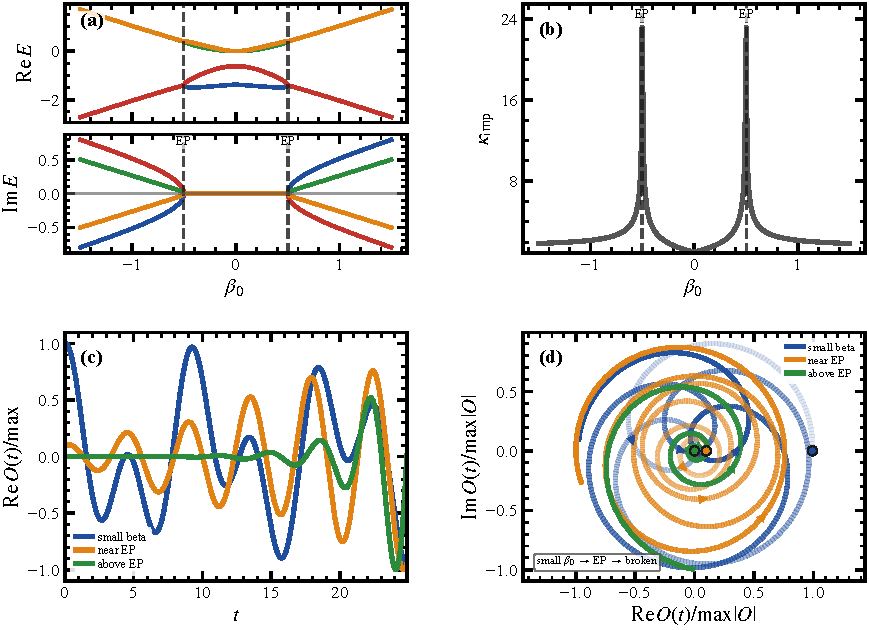
\includegraphics[width=0.86\linewidth,height=0.70\textheight,keepaspectratio]{Fig1.pdf}
\caption{%
\textbf{Full $4\times4$ non-Hermitian impurity kernel: spectrum, condition number, and real-time dynamics.}
All panels use the gauge-fixed frozen-kernel convention $\tb=|\gb|r$ with
$\epsilon_\xi=-U/2=-1.0$, $U=2.0$, and $T_{\rm b}=0.1$.
The plotted eigenvalues and eigenvectors are computed from the full rotated
$4\times4$ kernel of Eq.~(\ref{eq:Htilde}), not from the isolated impurity block.
\textbf{(a)} Real and imaginary parts of the four eigenvalues of
$\Htilde(k=0)$ versus $\gb$.  The representative finite-drive local EPs occur at
$|\gb|\simeq0.50$; double-root tracking gives
$\beta_{0,{\rm proj}}^{\rm EP}=0.4975$, while the discrete grid peaks at the adjacent point
$\beta_0=0.5025$ ($\Delta\beta_0=0.0075$).
\textbf{(b)} Condition number $\keff=\|R\|\,\|R^{-1}\|$,
using the same eigenvector normalization throughout the scan.  The finite-
$|\gb|$ peaks locate eigenvector coalescence; the origin is a normal degeneracy
and is not interpreted as an EP.
\textbf{(c)} Survival-amplitude dynamics for representative points below, at,
and above the EP, plotted on a common solver time window.
\textbf{(d)} Corresponding phase portraits.  The change from oscillatory motion
to critical coalescence and then to broken-regime overdamped response is the
time-domain signature of the $4\times4$ finite-drive EP.
}
\label{fig:full_H}
\end{figure}

\begin{figure}[t]
\centering
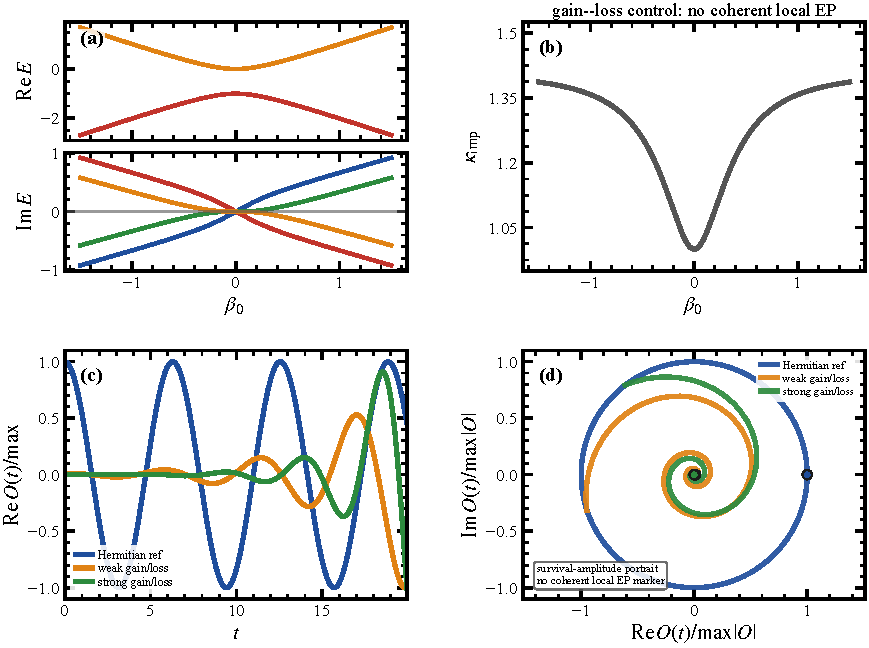
\includegraphics[width=0.86\linewidth,height=0.70\textheight,keepaspectratio]{Fig2.pdf}
\caption{%
\textbf{Full $4\times4$ relative gain--loss-only control.}
The same impurity-level convention is used as in Fig.~\ref{fig:full_H},
$\epsilon_\xi=-U/2=-1.0$ with $U=2.0$ and $T_{\rm b}=0.1$, but the coherent
local splitting/flip channel is switched off.  This isolates passive relative
gain--loss and bath dressing from the coherent impurity-EP mechanism.
\textbf{(a)} Real and imaginary parts of the four eigenvalues of the frozen
$4\times4$ kernel.
\textbf{(b)} Condition-number diagnostic.  Any residual structure is a
passive non-Hermitian bath-dressing diagnostic and is not interpreted as a
coherent finite-drive local impurity EP.
\textbf{(c)} Survival-amplitude dynamics for the Hermitian reference, weak
relative gain--loss, and strong relative gain--loss cases, plotted on a common time window.
\textbf{(d)} Phase portraits for the same three cases.  These trajectories are
shown in a normalized or co-decaying representation; they should not be read as
conservation of the Euclidean norm of the isolated relative gain--loss block.
}
\label{fig:flip0}
\end{figure}

Unless stated otherwise, the final numerical figures use the uniform local-moment convention
\begin{equation}
\epsilon_\xi=-U/2=-1.0,
\qquad U=2.0,
\qquad T_{\rm b}=0.1,
\label{eq:numerical_convention_final}
\end{equation}
with the gauge-fixed projected scale $\tb=|\gb|r$.  The projected double-root value is $\beta_{0,{\rm proj}}^{\rm EP}=0.4975$; the discrete condition-number grid peaks at the adjacent point $\beta_0=0.5025$.  Figure~\ref{fig:full_H} displays the corresponding pair at $|\gb|\simeq0.50$.

Figures~\ref{fig:full_H} and~\ref{fig:flip0} display the
dynamical fingerprints of the EP-active projected impurity block and of
the relative gain--loss-only diagnostic limit, respectively.
In the projected Kondo-regime kernel
($\epsilon_\xi=-1.0=-U/2$, $U=2.0$, $T_{\rm b}/T_K<1$), the representative
coefficients place a symmetric local EP pair at $|\gb|\simeq0.5$,
accompanied by a condition-number peak and by a crossover from
oscillatory to overdamped local dynamics.
Removing the coherent splitting channel ($\gm=0$, Fig.~\ref{fig:flip0})
removes the coherent local impurity EP mechanism.  The remaining
passive relative gain--loss dynamics is retained only as a diagnostic contrast:
it should not be interpreted as a separate positive-screening Kondo
scale enhancement.

\paragraph{Condition-number convention.}
All condition numbers shown below are computed from the Euclidean
right-eigenvector matrix of the full $4\times4$ channel-projected
kernel at the plotted $k$ slice, using a single normalization
convention for all values of \(\gb\).  We use
\(\keff\) to locate finite-\(|\gb|\) eigenvector coalescence and to
track the distance to the EP.  Its absolute magnitude is not used as a
standalone physical observable or as an independent definition of the
Kondo scale; the physical diagnostics are the spectral line shapes,
low-energy scale estimates, occupied fluctuation--dissipation-relation (FDR)-weighted spectra, and frozen
channel-projected amplitudes extracted with the same gauge-invariant
convention \(\tb=|\gb||b_c|\).

\subsection{Phase-Selective EP Enhancement}

\begin{figure*}[!t]
\centering

\includegraphics[width=0.78\textwidth,height=0.42\textheight,keepaspectratio]{Fig3.pdf}
\caption{%
\textbf{Compact frozen regime diagnostics: scales, peak merging, three-regime
spectra, and peak tracking.}
All panels use $\epsilon_\xi=-U/2=-1.0$, $U=2.0$, and the gauge-fixed scale
$\tb=|\gb|r$.  The positive-branch EP marker is
$\beta_{0,{\rm proj}}^{\rm EP}=0.4975$ in the plotted scan.
\textbf{(a)} Independent SBMF spectral-weight-transfer check.  The plotted
quantity is the positive spectral-weight transfer ratio
$\mathcal W_{\rm FSR}^{+}/\mathcal W_{\rm CP}^{+}$, normalized to the stable low-drive reference
$\beta_{0,{\rm ref}}=0.30$.  Here $\mathcal W_{\rm FSR}^{+}$ is the positive spectral
weight in a window around the shifted FSR/Kondo feature
$\omega_{\rm res}\simeq\mathrm{Re}\,\teps$, while $\mathcal W_{\rm CP}^{+}$ is the
corresponding positive weight in the central-peak window near $\omega=0$.
The faint points are raw window-integrated values and the solid line is a local
trend.  The ratio is meaningful only once the central-peak window carries
non-negligible positive weight, so the plotted range starts at the stable
low-drive plateau on which the reference is taken; at smaller $\beta_0$ the
central peak has not yet formed and the raw ratio is dominated by the
vanishing denominator (the full range is included in the exported data).
The diagnostic terminates at the negative-signed-weight onset
$\beta_0\simeq0.50$, i.e.\ at the EP, beyond which the signed response is
reported separately.  This construction avoids assigning a linewidth when
several peaks overlap or the signed projected response becomes
non-Lorentzian.  The analytic SW/BA
screening estimates are not overlaid here; they are compared with the same SBMF
transfer diagnostic on a common relative scale in the Supplemental Material.
\textbf{(b)} Peak-merging diagnostics extracted from the same frozen spectra:
the centroid separation, the upper- and lower-window widths, and the local
EP-distance $|s_{\rm eff}|$ are normalized to their panel maxima so the
coalescence/redistribution trend is visible even when the raw peaks are close.
\textbf{(c)} Broadened normalized retarded spectra for the screened
local-moment, resonant/mixed-valence, and high-temperature free-orbital
references.  When the same frozen retarded kernel is used, regime distinctions
come from $T_{\rm b}/T_K$ and from the occupied FDR-weighted spectrum rather than from
$A(\omega)$ alone.
\textbf{(d)} Peak positions versus $\gb$.  The reference line is
$\mathrm{Re}(\teps)=-1.0000$.  In the scan, the upper-window centroid ranges
from $-1.60\times10^{-2}$ to $1.63\times10^{-1}$, while the lower-window
centroid ranges from $-1.181$ to $-0.709$; the apparent peak separation is
largest near the EP because the signed frozen spectral response is strongly
non-Lorentzian there.
}
\label{fig:regimes}
\end{figure*}

Figure~\ref{fig:regimes} should be read as a compact frozen
channel-projected spectral diagnostic, not as a full finite-temperature SBMF
phase diagram.  The condition-number and $T_{\rm b}/T_K$ regime classifiers are
discussed in the text and caption rather than assigned separate panels.  Panel
(a) deliberately shows only the non-circular SBMF positive
spectral-weight-transfer diagnostic on its own normalized scale.  This avoids
forcing a window-integrated SBMF spectral measure and the analytic SW/BA
screening estimates to share an artificial absolute normalization.  The full
relative comparison of SW, BA, and the SBMF transfer ratio is given in
Supplemental Fig.~S3.  The exported data also include the peak-resolved HWHM
and re-solved FDR-window temperature diagnostics, but these are not used as main
scales because they can become ill-defined or non-monotonic when several peaks
overlap.

In the local-moment reference, particle-hole symmetry is imposed uniformly by
$\epsilon_\xi=-U/2=-1.0$ with $U=2.0$.  The Hubbard interaction is not inserted
as opposite $\pm U/2$ spin splittings in the $4\times4$ quasiparticle kernel.
The impurity-like spectral feature is therefore referenced to
$\omega\simeq\mathrm{Re}(\teps)=-1.0000$ in the frozen closure.  Moving
$\epsilon_\xi$ close to zero would move the coalescence toward the Fermi level,
but that would be a resonant or mixed-valence reference rather than the Kondo
local-moment convention used for the final figures.

% ============================================================
\section{Fluctuation-Dissipation Relation and Spectral Functions}
\label{sec:FDR}
% ============================================================

%        Fig. 4 uses the frozen-kernel reference Re(teps) generated by the
%        same figure pipeline.  Do not quote the older self-consistent value unless a
%        separate self-consistent closure is rerun and used for the figure.
\begin{figure}[t]
\centering

\includegraphics[width=0.90\linewidth,height=0.72\textheight,keepaspectratio]{Fig4.pdf}
\caption{%
\textbf{Bath-controlled FDR, eigenmode diagnostic, and physical spectral response.}
The uniform impurity convention is $\epsilon_\xi=-U/2=-1.0$, $U=2.0$, and
$T_{\rm b}=0.1$.  The bath-based FDR construction is the physical one used for
occupations and SBMF self-consistency.
\textbf{(a)} Impurity and bath FDR ratios obtained from
$G^<_{\rm phys}=f_{\rm FD}(\omega)[G^R-G^A]$ on spectral support.  Both follow
$f_{\rm FD}(\omega)$; in the exported diagnostic file the maximum residual of
the bath-constructed ratio from $f_{\rm FD}$ is below $10^{-12}$.
\textbf{(b)} Absolute FDR residual for the bath-constructed physical ratio;
the exported diagnostic gives a maximum residual below $10^{-12}$.
\textbf{(c)} Eigenmode-based ratio obtained by assigning occupations to
non-Hermitian eigenmodes.  This object is nonthermal and is shown only as a
nonnormality/eigenbasis diagnostic; it is not used in the saddle-point equations
or in the physical FDR analysis.
\textbf{(d)} Physical impurity spectral response with the Fermi level
$\omega=0$, the frozen impurity reference $\mathrm{Re}(\teps)=-1.0000$, and the
observed spectral peak marker.  When the frozen kernel is instead evaluated on
the PT-broken side, a negative signed response should be reported explicitly as
a causality diagnostic, not as a positive physical DOS.
}
\label{fig:FDR}
\end{figure}

For a non-Hermitian system, two inequivalent constructions of
$G^<$ arise and it is essential to distinguish them.
Figure~\ref{fig:FDR} separates these objects explicitly.  The impurity and
bath FDR ratios constructed from the reservoir self-energy follow the same
thermal Fermi function on spectral support.  The eigenmode-based construction
is displayed in a separate diagnostic panel because it is not a bath-imposed
distribution function; deviations of this diagnostic are therefore not a
physical violation of the fluctuation--dissipation relation.

\paragraph{Bath-based construction (physical).}
The physical lesser Green's function is fixed by the thermal bath
self-energy.  For a bilinear impurity--bath coupling,
\begin{equation}
\Gless_{\rm phys}(\omega)
=
\Gret(\omega)\,\Sigma^<_{\rm bath}(\omega)\,\Gadv(\omega).
\label{eq:Gless_physical_fdr}
\end{equation}
If the bath is thermal, then
\begin{equation}
\Sigma^<_{\rm bath}(\omega)
=
f(\omega)
\left[
\Sigma^R_{\rm bath}(\omega)-\Sigma^A_{\rm bath}(\omega)
\right].
\label{eq:bath_selfenergy_fdr}
\end{equation}
Combining this with the Dyson identity for the bath-induced
broadening gives
\begin{equation}
\Gless_{\rm phys}(\omega)
=
f(\omega)\,[\Gret(\omega)-\Gadv(\omega)].
\label{eq:impurity_fdr_inherited}
\end{equation}
Thus the physical impurity FDR is inherited from the reservoir and is
the $G^<$ used in the SBMF self-consistency.

\paragraph{Eigenmode-based construction (comparison).}
$\Gless_{\rm eig}=iR\,\mathrm{diag}(f(\mathrm{Re}\,\mathcal E_n))
\,L^\dagger$ assigns Fermi occupations $f(\mathrm{Re}\,\mathcal E_n)$
to the non-Hermitian eigenvalues $\mathcal E_n$.
Because the eigenvalues are complex, this construction does not
correspond to the thermal occupations imposed by the bath.
Consequently $\Gless_{\rm eig}$ is not interpreted as a physical
distribution function.  It is retained only as an auxiliary diagnostic
of the nonorthogonal eigenbasis and is not used in the SBMF
self-consistency or in the physical FDR analysis.

\paragraph{Impurity spectral function.}
The impurity spectral function is evaluated from the retarded and
advanced Green's functions as
\begin{equation}
A_{\rm imp}(\omega)
=
-\frac{1}{2\pi}\,
\mathrm{Im}\,\mathrm{Tr}
[\Gret(\omega)-\Gadv(\omega)]_{\rm imp}.
\label{eq:DOS}
\end{equation}
We use this bath-consistent construction throughout the spectral
analysis.  In contrast, using only
\(-\mathrm{Im}\,\mathrm{Tr}\,\Gret/\pi\) can introduce spurious
features from relative-kernel poles in a non-Hermitian representation.  The
spectral results below are therefore computed with the same retarded,
advanced, and bath-controlled lesser functions used in the
self-consistency.

\paragraph{Gauge convention for spectral functions.}
The physical self-energy from the coarse-graining is first decomposed into
a common bath shift/damping, the passive $\PT$ core of Eq.~(\ref{eq:passive_PT_core}),
and the Kramers--Kronig detuning of Eq.~(\ref{eq:relative_detuned_kernel}).
The off-shell auxiliary sector supplies the real spin-odd shift, while the
energy-dependent Dirac bath converts this shift into the relative
spin-dependent width $\Gamma_{\rm PT}$.  The
effective Hamiltonian is therefore written in terms of the real,
gauge-invariant amplitude $\tb=|\gb||b_c|$ and the projected channels
$\Gpt=\cGm\tb$, $\Deff=\Dzero+\cDl\tb$, and $\Veff=\cV\tb$.
The phase of the auxiliary slave-boson field is not used separately
in spectral calculations.  With this convention, the same $\Hss$ is
used for eigenvalues, condition numbers, and spectral functions, and
no observable is attributed to the gauge-dependent phase of $b_c$.

% ============================================================
\section{Real-Time Dynamics}
\label{sec:dynamics}
% ============================================================

The real-time diagnostic is the complex survival amplitude
\begin{equation}
O(t)=\langle d_\uparrow|e^{-iHt}|d_\uparrow\rangle ,
\label{eq:survival_amplitude}
\end{equation}
evaluated for the same gauge-fixed frozen kernel used in the spectral
plots.  We show both $\mathrm{Re}\,O(t)$ and the phase portrait
$[\mathrm{Re}\,O(t),\mathrm{Im}\,O(t)]$.  This is a non-unitary
propagator diagnostic of the local EP; it is not used as a normalized
thermal expectation value.  For Fig.~\ref{fig:full_H}(c),(d) we use
$\epsilon_\xi=-U/2=-1.0$, $U=2.0$, $T_{\rm b}=0.1$, and
$\beta_{0,{\rm proj}}^{\rm EP}\approx0.5$.  The evolution shows a direct dynamical
signature of the EP:

\begin{itemize}
\item \emph{Below EP} ($\gb<\beta_{0,{\rm proj}}^{\rm EP}$, local splitting real):
  eigenvalues are non-degenerate; the evolution shows underdamped
  oscillations with a frequency set by $\mathrm{Re}(E_+-E_-)=2\mathrm{Re}\,s$
  and a decay rate set by $\mathrm{Im}(E_\pm)$.

\item \emph{Above EP} ($\gb>\beta_{0,{\rm proj}}^{\rm EP}$, local splitting imaginary):
  eigenvalues have opposite imaginary parts; the gain mode
  dominates and the evolution shows overdamped decay.

\item \emph{Without flip} ($\gm=0$, Fig.~\ref{fig:flip0}):
  the isolated relative gain--loss block has eigenvalues
  $\teps\pm i\Gpt$ and is therefore in the broken sector for
  $\Gpt\neq0$.  The plotted bounded trajectories are normalized or
  co-decaying diagnostics of the full bath-coupled kernel, not evidence
  for conservation of the Euclidean norm.
\end{itemize}

The contrast between the normalized no-flip diagnostic and the spiraling
dynamics with coherent splitting demonstrates that both projected
impurity channels of $\Htilde$---the coherent splitting $\Deff$ and the
relative decay channel $i\Gpt$---are necessary for the full finite-drive
EP structure.  In the channel-projected parametrization, these channels are measured
relative to the common scale $\tb$ but should be viewed as distinct
projected self-energy components.  Equality of their coefficients is a
symmetric representative limit, not a symmetry requirement.

% ============================================================
\section{Biorthogonal Bethe Ansatz}
\label{sec:BA}
% ============================================================

The saddle-point treatment of Sec.~\ref{sec:mf} motivates the
gauge-invariant scale $\tb=|\gb||b_c|$ and the renormalized level
$\teps$.  The Bethe-Ansatz analysis below is a frozen effective-model
diagnostic: $\gm$ denotes the coherent impurity splitting/flip channel,
while $\gb$ denotes the projected relative gain--loss channel in the minimal
frozen notation.  The general projected description is
$\Gpt=\cGm\tb$, $\Deff=\Dzero+\cDl\tb$, and $\Veff=\cV\tb$.
The local EP is controlled by the competition between $\Gpt$ and
$\Deff$, while $\Veff$ controls bath coupling and the positive
screening hybridization.
The diagonal hybridization structure [property~(i) of
Sec.~\ref{sec:rotation}] is the key that makes the frozen-$\tb$
problem analytically tractable: it forces the two-body $S$-matrix to be
block-diagonal ($S^{LR}=S^{RL}=0$), providing the channel separation used in the Bethe-Ansatz
construction of the frozen effective model.
For the frozen diagnostic phase diagram, $\gb$ (gain/loss amplitude)
and $\gm$ (coherent flip amplitude) are kept as independent
projection channels.  Their equality is a special symmetric
representative, not a general consequence of the slave-boson saddle.
The frozen-BA approximation is used only as a low-energy analytic
screening diagnostic, most directly when $T_{\rm b}\ll T_K$ and hybridization
fluctuations about the saddle point are small.

\subsection{Block-Diagonal $S$-Matrix from Diagonal Hybridization}

The diagonal hybridization [property~(i) of Sec.~\ref{sec:rotation}]
is the key that makes the frozen effective model channel-separated.
Because $\tilde{d}_+$ couples only to $c_{k+}$ and $\tilde{d}_-$
only to $c_{k-}$, the two-body scattering is channel-diagonal:
bath $+$ electrons can only scatter from the $\tilde{d}_+$
impurity state and vice versa.
The internal relative channel $i\gb$ is an excitation that mixes
the two impurity states, but it does not connect incoming bath $+$
electrons to outgoing bath $-$ electrons.  This follows because the
hybridization vertices preserve the bath channel index, so impurity
mixing does not induce cross-channel propagation of bath electrons.
This is verified by the two-body contact algebra
(Supplemental Material): the off-diagonal scattering
amplitudes $e_{+-}$ and $e_{-+}$ satisfy homogeneous equations
[Eqs.~(G2) and~(G4)] with no external bath
source terms.
Together with the density-density interaction $H_U=Un_{d+}n_{d-}$
(which preserves channel labels), this gives the block-diagonal $S$-matrix:
\begin{equation}
S^{LR}=S^{RL}=0,\qquad
S_{\rm tot}=\begin{pmatrix}S^{RR}&0\\0&S^{LL}\end{pmatrix}.
\label{eq:Stot}
\end{equation}
The biorthogonal impurity problem therefore separates into
independent right and left sectors, which is the structural input
used for the Bethe-Ansatz construction below.

\subsection{Renormalized Contact Denominators and Breit--Wigner $S$-Matrix}

The two-body contact algebra (Supplemental Material) gives
the renormalized denominators through the relative channel $\gb$:
\begin{equation}
\mathfrak a = \teps+\gm-E,\quad \mathfrak b = \teps-\gm-E,
\label{eq:ab_bare}
\end{equation}
\begin{equation}
\tilde{\mathfrak a}=\mathfrak a+\frac{\gb^2}{\mathfrak b},\qquad
\tilde{\mathfrak b}=\mathfrak b+\frac{\gb^2}{\mathfrak a}.
\label{eq:atilde}
\end{equation}
Here $\mathfrak a$ and $\mathfrak b$ are energy denominators for the $\tilde{d}_+$
and $\tilde{d}_-$ impurity levels respectively; the bath
dispersion $\varepsilon_{c,\pm}(k)$ enters the contact equations
through the bath wavefunctions $\Phi_\pm$, not through $\mathfrak a$ or $\mathfrak b$.
Each diagonal block of the $S$-matrix takes the Breit--Wigner
form:
\begin{equation}
S^{XX}_{\eta\eta}(k)
=\frac{k-\tilde\epsilon_{d,\eta}-i\tilde\Gamma_\eta}
      {k-\tilde\epsilon_{d,\eta}+i\tilde\Gamma_\eta},
\quad X\in\{R,L\},\;\eta\in\{+,-\},
\label{eq:Ssoln}
\end{equation}
where $\tilde\epsilon_{d,\eta}=\epsilon_{d,\eta}+\Lambda_\eta^{\rm PV}$ is the
bath-shifted impurity level with one-body shift
$\Lambda_\eta^{\rm PV}=(V_\eta)^2\sum_k(\epsilon_{d,\eta}-\varepsilon_{c,\eta}(k))^{-1}$.
For reciprocal Hermitian hybridization the resonance width is
$\tilde\Gamma_\eta=\pi\rho_{b,\eta}(0)|V_\eta|^2$.  In a genuinely
non-Hermitian or nonreciprocal channel this is replaced by the
biorthogonal product
\begin{equation}
\tilde\Gamma_\eta^{\rm bio}
=
\pi\rho_{b,\eta}(0)V_\eta^R V_\eta^L .
\label{eq:Gamma_bio_product}
\end{equation}
The density $\rho_{b,\eta}(0)$ used here is the local radial-channel
density of states of the frozen channel-projected effective model,
evaluated at the active resonance after the chiral rotation and
low-energy linearization.  It is not the bare two-dimensional Dirac
point density $\rho_{\rm bath}(\omega)\sim |\omega|/\lambda^2$, which
vanishes at the undoped Dirac point.  In the frozen BA diagnostic we
work in a finite scattering window where $\rho_{b,\eta}$ is slowly
varying and may be replaced by the constant
$\rho_{b,\eta}(0)\simeq1/k_{\rm max}$.  The full numerical spectral
calculations retain the bath dispersion explicitly.

\subsection{Integrability via Yang--Baxter Equation}
\label{sec:YBE}

Because the diagonal hybridization [Eq.~(\ref{eq:Htilde})]
decouples the $+$ and $-$ channels completely, the $S$-matrix in
each diagonal block is a \emph{scalar} Breit--Wigner
[Eq.~(\ref{eq:Ssoln})].  Scalar $S$-matrices trivially satisfy the
Yang--Baxter equation: for c-number $S^X_{\eta\eta}(k)$, the
three-body relation
\begin{align}
S^X_{\eta\eta}(k_1{-}k_3)\,S^X_{\eta\eta}(k_2{-}k_3)\,S^X_{\eta\eta}(k_1{-}k_2)
\nonumber\\
=S^X_{\eta\eta}(k_1{-}k_2)\,S^X_{\eta\eta}(k_2{-}k_3)\,S^X_{\eta\eta}(k_1{-}k_3)
\label{eq:YBE_scalar}
\end{align}
holds identically by commutativity of scalar multiplication,
establishing channel-separated scattering in the frozen
model.

Supplemental Material gives the same statement in the contact-projector
notation.  Since each frozen block is a scalar Breit--Wigner amplitude,
YBE factorization follows from channel separation and scalar
commutativity alone.  No additional Baxterization functional equation is
required.  Bath dispersions enter only as diagonal one-body phases in
the Bethe equations and do not spoil factorization.

%   captions rewritten to reflect the corrected figure content
%   (eta_phys used, so Im(mu^R) is finite everywhere; panel (c) shows
%   channel splitting, not L-R distance).
\begin{figure}[t]
\centering

\includegraphics[width=\linewidth]{fig5_rapidities.pdf}
\caption{%
\textbf{Biorthogonal BA rapidities and EP structure.}
Three layers per panel represent distinct levels of physics
($\epsilon_\xi=-U/2=-1.0$, $U=2.0$, $\gm=\gb=0.5$ at bare EP,
$\lambda=0.50$, $k_{\rm max}=\pi/4$,
D-SOC$^2$ form factor $F=1-(\lambda/k_{\rm max})^2\approx0.595$).
Vertical red dashed lines mark the bare EP at $|\gb|=\gm=0.5$.
\emph{Layer~1 (thick black)}: bare $h_d$ eigenvalues
$E_\pm^{\rm bare}=\teps\pm s$, $s=\sqrt{\gm^2-\gb^2}$.
This is the only layer with a genuine EP (at $\gb=\gm$, where $s=0$).
\emph{Layer~2 (grey)}: $U$-corrected levels
$\teps\pm\seff$ from the quartic (Supplemental Material);
$\seff>0$ for all $\gb$ when $U>0$ and $F(\lambda)>0$ (EP avoided).
\emph{Layer~3 (blue circles: bare $s$; orange squares: $s_{\rm eff}$)}:
Bethe-dressed rapidities $\mur^{R,U}_\pm=(\teps\pm\seff)+\Lambda_\pm^{\rm PV}$
using the physical S-matrix resonance width
$\tilde\Gamma_\eta=\pi V_\eta^2\rho_{b,\eta}(0)=\pi\gb^2/k_{\rm max}$
(for this frozen diagnostic $r=1$, so $V_\eta=\tb=|\gb|$) in the bath shift $\Lambda_\pm^{\rm PV}$;
$\mur^L = (\mur^R)^*$ by $\PT$ symmetry.
\textbf{(a)} Real parts vs $\gb$: $\mathrm{Re}\,\mur^R=\mathrm{Re}\,\mur^L$
by $\PT$ symmetry; only the bare $U=0$ layer coalesces at the bare EP, while the $U>0$ layers remain split.
\textbf{(b)} Imaginary parts vs $\gb$: $\mathrm{Im}\,\mur^R=-\tilde\Gamma_{\rm phys}
=-\pi\gb^2/k_{\rm max}$
is the physical bath decay width, finite everywhere for all $\gb$.
$\mathrm{Im}\,\mur^L=-\mathrm{Im}\,\mur^R$ by $\PT$ (mirror symmetry).
The imaginary part is \emph{not} an EP diagnostic; see panel~(c).
\textbf{(c)} Channel splitting $|\mur^{R(+)}-\mur^{R(-)}|$
(log scale): the genuine EP diagnostic (text after Eq.~\ref{eq:BAaux}).
Three reference layers are shown: $2|s|$ (Layer~1, black), $2|\seff|$
(Layer~2, grey), and the bath-dressed splitting (Layer~3, coloured).
Bare $s$ touches zero at $\gb=\gm$; $U$-corrected $\seff$ stays
finite (EP regularised by interactions).
\textbf{(d)} Biorthogonal width $\tilde\Gamma_{\rm bio}=\gb^2/s$
vs $\gb$ (log scale): diverges at the bare EP ($s\to0$),
driving the biorthogonal norm divergence and BA-kernel nonnormality enhancement; regularised to $\gb^2/\seff$ by interactions
($U>0$, orange dashed), remaining finite everywhere.
}
\label{fig:bethe}
\end{figure}

\begin{figure}
\centering

\includegraphics[width=\linewidth]{fig6_phasediag.pdf}
\caption{%
\textbf{EP-boundary diagnostic controlled by the SOC form factor.}
Color: $\mathcal{D}_{\rm EP}(U,\lambda)=\gm^2-C_FU^2F(\lambda)$,
derived in the Supplemental Material in the adopted dimensionless
normalization $C_F=1$ and evaluated at the bare control point
$\gb=\gm$.
Positive (red): relative $\PT$-unbroken ($\mathcal{D}_{\rm EP}>0$); negative
(blue): relative $\PT$-broken ($\mathcal{D}_{\rm EP}<0$).
The thick black curve is the local EP-boundary diagnostic
$\mathcal{D}_{\rm EP}(U,\lambda)=0$.
Horizontal lines mark the SOC values used in Fig.~\ref{fig:bethe}:
dashed $\lambda=0.50$, dotted $\lambda=k_{\rm max}=\pi/4$.
\textbf{(a)} Gaussian form factor $F=e^{-(\lambda/k_{\rm max})^2}$:
interactions $U$ regularise the EP for all $\lambda$; the EP
boundary curves to large $U$ as $\lambda\to k_{\rm max}$.
\textbf{(b)} D-SOC$^2$ form factor
$F=\max(1-(\lambda/k_{\rm max})^2,\,0)$: at $\lambda=k_{\rm max}$,
$F=0$ exactly (orange dotted line), so $U$ cannot regularise
the EP regardless of interaction strength---producing the sharp
vertical wall in this analytic diagnostic.  The figure illustrates the
model dependence of the interaction-induced impurity-sector EP shift; it
is not used as a standalone many-body phase diagram or an independent
determination of the Kondo scale.
}
\label{fig:phasediag}
\end{figure}

\subsection{Bethe Ansatz Equations}

The charge rapidities $\{k_j^R\}$ in the right sector satisfy:
\begin{equation}
e^{ik_j^R\mathcal{L}}
=\prod_{\ell\neq j}S^{RR}(k_j^R-k_\ell^R)
\prod_{\eta,a}
\frac{\mur^{R(\eta)}_a-k_j^R+\tilde\epsilon_{d\eta}
      +i\tilde\Gamma^R_\eta/2}
     {\mur^{R(\eta)}_a-k_j^R+\tilde\epsilon_{d\eta}
      -i\tilde\Gamma^R_\eta/2},
\label{eq:BAright}
\end{equation}
and the auxiliary rapidities $\{\mur^{R(\eta)}_a\}$ satisfy:
\begin{multline}
\prod_j
\frac{\mur^{R(\eta)}_a-k_j+\tilde\epsilon_{d\eta}
      +i\tilde\Gamma^R_\eta/2}
     {\mur^{R(\eta)}_a-k_j+\tilde\epsilon_{d\eta}
      -i\tilde\Gamma^R_\eta/2}
\\
=\prod_{b\neq a}
\frac{\mur^{R(\eta)}_a-\mur^{R(\eta)}_b
      +i\tilde\Gamma^R_\eta}
     {\mur^{R(\eta)}_a-\mur^{R(\eta)}_b
      -i\tilde\Gamma^R_\eta}.
\label{eq:BAaux}
\end{multline}
Left-sector equations follow by $R\to L$.  Written with symmetric
$\pm i\tilde\Gamma_\eta/2$ shifts, these equations reduce to the standard
Hermitian Anderson impurity quantization conditions when
$V_\eta^R=V_\eta^L$ and the relative non-Hermitian channel is set to zero.
The bare $U=0$ EP manifests in the BA through the channel splitting
$2|s|\to0$ at $\gb=\gm$.  For $U>0$ and $F(\lambda)>0$, the
interaction-corrected splitting $2\seff$ remains finite and represents
an avoided coalescence at the same bare control point
(the R--L distance $|\mur^R-\mur^L|=2\tilde\Gamma$ is nonzero
everywhere and is not an EP diagnostic; see also
Refs.~\cite{garcia2022jordan,yi2022novel}).
The dressed rapidities $\mur^{R/L}_\pm$ presented in
Fig.~\ref{fig:bethe} encode the full pseudo-Hermitian structure:
the three-layer picture---bare hd eigenvalues, interaction-corrected
$\teps\pm\seff$, and Bethe-dressed $\mur^{R,U}_\pm$---demonstrates
how interactions replace the bare coalescence by an avoided one, with the
channel splitting serving as the quantitative EP-distance diagnostic across
all parameter regimes.


\subsection{Frozen-model BA scattering kernel and screening-scale estimate}
\label{sec:frozen_TBA_scale}

The frozen Bethe-Ansatz (BA) construction gives a channel-diagonal
Breit--Wigner scattering amplitude.  In what follows we use the logarithmic
derivative of this frozen two-body scattering phase to define an
integrability-based kernel and then match its dimensionful scale to the same
microscopic Anderson channel used in the Schrieffer--Wolff reduction.  The
result is therefore a BA-kernel screening-scale estimate for the frozen
effective model, rather than a full thermodynamic Bethe-Ansatz determination
of the Kondo temperature:
\begin{equation}
S_{\eta}(k)=
\frac{k-\tilde{\epsilon}_{d,\eta}-i\tilde{\Gamma}_{\eta}}
{k-\tilde{\epsilon}_{d,\eta}+i\tilde{\Gamma}_{\eta}},
\qquad \eta=\pm .
\label{eq:S_frozen_TBA}
\end{equation}
The rapidity matching used below follows the usual frozen
Anderson--Kondo scattering construction: the charge rapidity is measured from
the dressed impurity level, $u=k-\tilde\epsilon_{d,\eta}$, and the
logarithmic derivative of the Breit--Wigner phase shift gives the kernel in
Eq.~(\ref{eq:TBA_kernel_frozen}).  The phase-shift kernel fixes the scattering
structure but does not by itself determine a unique thermodynamic energy
scale.  We therefore set the dimensionful scale by matching the same frozen
channel to the Schrieffer--Wolff exchange.  In this construction the imaginary
parts and coalescence of the biorthogonal rapidities diagnose the EP structure;
they are not identified directly with $T_K$.
At the uniform particle-hole convention used in the final figures,
$\epsilon_\xi=-U/2=-1.0$ and $U=2.0$, the two virtual charge denominators are
both unity,
\begin{equation}
|\tilde\epsilon_d|^{-1}+|\tilde\epsilon_d+U|^{-1}=1+1=2,
\label{eq:PH_denominator_numeric}
\end{equation}
so the PH-symmetric exponent reduces to
$-\pi/(4\chi_K\tilde\Gamma_{\eta}^{\rm bio})$ in the dimensionless units of
the frozen scale estimate.  This is the rapidity-to-Anderson matching used for
the SW/BA-kernel relative comparison of Supplemental Fig.~S3.

For a reciprocal Hermitian Anderson channel,
\begin{equation}
\tilde{\Gamma}_{\eta}=\pi\rho_{b,\eta}(0)|V_{\eta}|^2,
\label{eq:Gamma_Hermitian}
\end{equation}
while a non-Hermitian or nonreciprocal channel is described by the
biorthogonal product
\begin{equation}
\tilde{\Gamma}_{\eta}^{\rm bio}
=\pi\rho_{b,\eta}(0)V_{\eta}^{R}V_{\eta}^{L}.
\label{eq:Gamma_TBA_bio}
\end{equation}
Only positive-real-part screening eigenvalues of the corresponding
exchange matrix are interpreted as Kondo screening channels.

Spin--orbit coupling (SOC) enters the frozen scale through the active
channel width,
\begin{equation}
\tilde{\Gamma}_{\eta}^{\rm bio}(\lambda)
=\pi\rho_{b,\eta}(0;\lambda)
V_{\eta}^{R}(\lambda)V_{\eta}^{L}(\lambda) .
\label{eq:SOC_width_TBA}
\end{equation}
The channel density of states contains the Rashba-split velocity
Jacobian,
\begin{equation}
\rho_{b,\eta}(0;\lambda)
=
\sum_{k_\ast}
\frac{\mathcal{J}_{2}(k_\ast)}
{\left|\partial_k\varepsilon_{\eta}(k;\lambda)
\right|_{k=k_\ast}},
\qquad
\varepsilon_{\eta}(k_\ast;\lambda)=0,
\label{eq:SOC_DOS_velocity}
\end{equation}
where $\mathcal{J}_{2}(k)=k/(2\pi)$ in two dimensions.  Unless the
real part of the bath self-energy is explicitly retained,
$\tilde\epsilon_{d,\eta}$ is kept as the frozen impurity level and the
explicit SOC dependence is collected in
$\tilde\Gamma_{\eta}^{\rm bio}(\lambda)$.  If such a real
shift is retained, one replaces
\begin{equation}
\tilde{\epsilon}_{d,\eta}
=\epsilon_d+\mathrm{Re}\,\Sigma_{\eta}^{R}(0;\lambda).
\label{eq:SOC_epsilon_shift}
\end{equation}

With $u=k-\tilde\epsilon_{d,\eta}$, the logarithmic derivative of
Eq.~(\ref{eq:S_frozen_TBA}) gives the Lorentzian frozen BA-kernel,
\begin{align}
K_\eta(u)
&=\frac{1}{2\pi i}\frac{d}{du}\ln S_\eta(u)
\notag\\
&=\frac{1}{\pi}\frac{\tilde\Gamma_\eta}
{u^2+\tilde\Gamma_\eta^2},
\qquad
\int du\,K_\eta(u)=1 .
\label{eq:TBA_kernel_frozen}
\end{align}
This kernel fixes the frozen scattering phase.  The associated
screening-scale estimate follows only after matching to the microscopic
Anderson exchange; no separate identification of $T_K$ with the imaginary
weight of a Bethe string is required in the present frozen-kernel construction.  The frozen
Schrieffer--Wolff exchange is
\begin{equation}
J_{\eta}^{\rm SW}=2|V_\eta|^2
\left[
|\tilde\epsilon_{d,\eta}|^{-1}
+|\tilde\epsilon_{d,\eta}+U|^{-1}
\right],
\label{eq:SW_exchange_frozen}
\end{equation}
so that
\begin{equation}
T_{K,\eta}^{\rm BA}
\simeq
D_{{\rm uv},\eta}
\exp\left[-\frac{\pi}
{2\chi_K\,\tilde\Gamma_\eta
\left(
|\tilde\epsilon_{d,\eta}|^{-1}
+|\tilde\epsilon_{d,\eta}+U|^{-1}
\right)}\right].
\label{eq:TK_BA_width}
\end{equation}
In the SOC-resolved non-Hermitian channel one reads
$\tilde\Gamma_\eta\to\tilde\Gamma_{\eta}^{\rm bio}(\lambda)$.
Thus SOC enhances or suppresses the frozen scale only by increasing or
decreasing the positive screening-channel width, or by an explicitly
included real level shift.

At particle-hole symmetry with no channel-dependent real shift,
$\tilde\epsilon_{d,\eta}=-U/2$, Eq.~(\ref{eq:TK_BA_width}) reduces to
\begin{equation}
T_{K,\eta}^{\rm BA}
\simeq
D_{{\rm uv},\eta}
\exp\left[-\frac{\pi U}
{8\chi_K\,\tilde\Gamma_{\eta}^{\rm bio}(\lambda)}\right].
\label{eq:TK_BA_PH}
\end{equation}
If a real channel shift
$\tilde\epsilon_{d,\eta}=-U/2+\eta s_\epsilon$ is retained, the
linear $\eta s_\epsilon$ terms from the empty and doubly occupied
virtual charge sectors cancel, giving for $|s_\epsilon|<U/2$
\begin{equation}
T_{K,\eta}^{\rm BA}
\simeq
D_{{\rm uv},\eta}
\exp\left[-\frac{\pi(U^2-4s_\epsilon^2)}
{8\chi_K\,\tilde\Gamma_{\eta}^{\rm bio}(\lambda)U}\right].
\label{eq:TK_BA_PH_shifted}
\end{equation}
As $|s_\epsilon|\to U/2$, the local-moment Schrieffer--Wolff estimate
breaks down and the system crosses into mixed-valence physics.

For a genuinely non-Hermitian channel, the scalar product
$V_\eta^RV_\eta^L$ replaces $|V_\eta|^2$.  A conventional screening
scale is then attached only to positive-real-part eigenvalues,
\begin{align}
T_K^{\rm BA,NH}
&=D_{\rm uv}\exp\left[-\frac{1}{\chi_K j_{\rm scr}}\right],
\label{eq:TK_BA_screening}\\
j_{\rm scr}
&=\max\left\{\operatorname{Re}j_\alpha:\;
 j_\alpha\in\operatorname{spec}(\rho_bJ^{\rm bio}),\;
 \operatorname{Re}j_\alpha>0\right\}.
\label{eq:j_scr_BA}
\end{align}
A negative or complex hybridization product can produce a frozen
non-Hermitian EP/crossover, but it is not by itself an enhanced
thermodynamic Kondo temperature.

Near an impurity EP that feeds a positive screening channel, the
biorthogonal residue may enhance the active width in the frozen estimate,
\begin{equation}
\tilde\Gamma_{\eta}^{\rm BA,EP}
=Z_\eta^{\rm bio}\tilde\Gamma_{\eta}^{\rm bio}(\lambda),
\qquad
1\le Z_\eta^{\rm bio}\le Z_{\rm max},
\label{eq:Gamma_bio_def}
\end{equation}
with the bounded diagnostic form
\begin{equation}
Z_\eta^{\rm bio}=
\min\left[Z_{\rm max},
\frac{s_{{\rm ref},\eta}}
{\max(|s_{\rm eff}|,s_{\rm floor})}\right].
\label{eq:Gamma_bio_bound}
\end{equation}
Here $s_{{\rm ref},\eta}$ is a smooth off-EP channel normalization,
$s_{\rm floor}>0$ is the causal/numerical infrared floor, and $Z_{\rm max}$
prevents a formal Jordan divergence from being interpreted as an observable.
For the plotted analytic curve we use $s_{{\rm ref},\eta}=0.375$,
$s_{\rm floor}=0.03$, and $Z_{\rm max}=25$.
Writing the nonsingular projection onto the screening channel as
$\mathcal A_\eta$, define
\begin{equation}
\mathcal J_\eta^{\rm eff}
=\mathcal A_\eta|V_\eta^RV_\eta^L|
\left(|\tilde\epsilon_{d,\eta}|^{-1}
+|\tilde\epsilon_{d,\eta}+U|^{-1}\right).
\label{eq:Jeta_eff}
\end{equation}
The corresponding frozen-model scale is
\begin{equation}
T_{K,\eta}^{\rm BA,EP}
\simeq
D_{{\rm uv},\eta}
\exp\left[-\frac{\pi|s_{\rm eff}|}
{2\chi_K\mathcal J_\eta^{\rm eff}}\right].
\label{eq:TK_BA_EP}
\end{equation}
Equation~(\ref{eq:TK_BA_EP}) is an analytic frozen-model scale, or
EP-distance diagnostic, not the exact thermodynamic Kondo temperature
of the full driven interacting problem.


% ============================================================
\section{Near-EP Low-Energy Scale Diagnostics}
\label{sec:kondo}
% ============================================================

Near the EP, the condition number
$\keff\sim C/|\seff|$ provides a diagnostic of eigenvector
nonorthogonality and of the associated redistribution of low-energy
spectral weight within the SBMF treatment.  In the conservative
interpretation used here, Eq.~(\ref{eq:TKep}) is a screening-eigenvalue
estimate rather than a universal expression for the exact Kondo
temperature.  The low-energy response is phase-selective: it is most visible
in the Kondo regime (Fig.~\ref{fig:regimes}) and is reduced both by
large SOC, which suppresses the overlap factor $F(\lambda)$ in
Supplemental Material, and by strong interaction-induced
regularisation, which increases $\seff$.
The diagnostic mechanism is the near-collinearity of the right
eigenvectors,
$|r_+\rangle\approx|r_-\rangle$ as $s\to0$, accompanied by the
corresponding growth of the dual norm.  Thus
$\keff=\|R\|\|R^{-1}\|$ tracks the distance to the EP and the
near-EP redistribution of impurity spectral weight, but it is not used
as a standalone proof of a universal Kondo-scale enhancement.  A
proper Kondo-temperature enhancement is claimed only when the EP-active
sector feeds a positive antiferromagnetic screening eigenvalue of
$\rho_bJ^{\rm bio}$.
The enhancement is exponential: SOC does not add a separate factor to
\(T_K\), but changes the screening width appearing in the denominator
of the Kondo exponent.  If the Rashba-split bath increases the active
channel density of states or the chiral hybridization product
\(V_\eta^R V_\eta^L\), then
\(\tilde\Gamma_\eta^{\rm bio}(\lambda)\) increases and the
negative exponent in \(T_{K,\eta}^{\rm BA}\) is reduced in magnitude.
Conversely, if SOC lowers the active density of states or suppresses
the form factor, the same expression suppresses the frozen Kondo
scale.  Near an impurity EP feeding a positive screening channel, the
biorthogonal residue further renormalizes the width as
\(\tilde\Gamma_{\eta}^{\rm BA,EP}
=Z_\eta^{\rm bio}\tilde\Gamma_\eta^{\rm bio}\), where $Z_\eta^{\rm bio}$ is the bounded diagnostic factor of
Eqs.~(\ref{eq:Gamma_bio_def})--(\ref{eq:Gamma_bio_bound}).  This gives an
additional EP-assisted increase of the frozen scale as the regularized
EP-distance is reduced, but not a literal divergent thermodynamic
Kondo temperature.

% ============================================================
\section{Conclusions}
\label{sec:conc}
% ============================================================

We have shown that a strictly Hermitian, periodically driven
quantum impurity coupled to a spin-orbit-split Dirac bath
develops emergent passive non-Hermitian behavior through a transparent
and controllable microscopic mechanism.  Bilinear Gaussian coarse
graining over off-shell angular-momentum harmonics produces a real
spin-odd coherent shift.  Embedding this shifted channel in the
energy-dependent retarded Dirac bath converts it into a spin-dependent
width.  After subtracting the common bath damping, the compensated relative kernel
contains the passive $\PT$ core of Eq.~(\ref{eq:passive_PT_core}), while the
Kramers--Kronig partner $\Dcoh\sigma_z$ acts as a causal detuning floor.
The gauge-invariant amplitude $\tb=|\gb||b_c|$ controls the projected
channel hybridization.

Four central and physically distinct results emerge:

First, the Hadamard rotation $U_2$ diagonalizes the hybridization
block exactly, producing $\tilde{d}_\pm$ channels that couple
exclusively to the $c_{k\pm}$ bath modes [Eq.~(\ref{eq:Htilde})].
This diagonal structure makes the two-body $S$-matrix block-diagonal
($S^{LR}=S^{RL}=0$), which is the origin of the channel-separated scattering
used in the frozen-model Bethe-Ansatz construction.

Second, the condition number $\keff\sim C/|\seff|$ shows a
phase-selective EP response within the SBMF treatment,
with the largest response in the Kondo regime and much weaker
responses in the resonant-level and free-orbital regimes
(Fig.~\ref{fig:regimes}).  The interaction $U$ renormalizes the
EP distance $\seff$ and keeps the condition number finite.  Thus
$\keff$ is used as a diagnostic of nonnormality and of the associated
low-energy scale diagnostics, rather than as a standalone proof of a
universal Kondo scale.
The sign difference of the passive relative gain--loss channel alone does not
split the Kondo scale, since the naive channel estimate depends on the
squared detuning.  Distinct channel scale estimates arise only when the
SOC-split bath or the self-consistent saddle produces unequal channel
widths or real detunings, as detailed in the Supplemental Material.  The
condition-number peaks in Figs.~\ref{fig:full_H}--\ref{fig:regimes}
are therefore interpreted as finite-$|\gb|$ EP diagnostics whose
response is strongest in the Kondo regime, rather than as a separate
universal ``$\tb\sim T_K$'' precursor criterion.

Third, SOC enters the screening-scale estimate through the
channel-resolved density of states, cutoff, chiral hybridization form factor,
and one-body level shift.  The frozen BA-kernel expression
$T_{K,\eta}^{\rm BA}(\lambda)$ should therefore be read as an
integrability-based low-energy diagnostic, matched to the Schrieffer--Wolff
channel, rather than as an independent exact thermodynamic identity.  Its
variation captures a combined SOC-projection and impurity-sector
nonnormality effect within the frozen effective model, not a universal
monotonic enhancement of $T_K$ with SOC.


The location of the exceptional point is also important for this
interpretation.  In the mechanism studied here the relevant EP is localized
in the effective impurity block and can modify the same positive screening
channel that enters the Schrieffer--Wolff exchange.  In that case an enhanced
biorthogonal residue may increase the corresponding frozen screening-scale
estimate.  An EP generated predominantly by the bath dispersion, reservoir
self-energy, or an extended bath sector need not feed the local exchange in
the same way.  Such a bath-induced EP may alter spectral, transport, or decay
properties without producing a comparable Kondo-scale enhancement.  The
connection between an EP and screening is therefore conditional on how the EP
projects onto the low-energy impurity screening channel.

Fourth, the driven impurity exhibits a shifted Friedel-type
resonance: the low-energy peak is referenced by
$\omega_{\rm res}\simeq\mathrm{Re}(\teps)\neq0$
[Eq.~(\ref{eq:omega_K})].
This shift is expressed in terms of the gauge-invariant amplitude
$|b_c|$, the spin-selective self-energy, and the renormalized
impurity level; it is not attributed to the phase of the auxiliary
slave-boson field.
For the frozen kernel plotted in Fig.~\ref{fig:FDR}, the reference
position is $\omega_{\rm res}\simeq\mathrm{Re}(\teps)=-1.0000$ at
$\epsilon_\xi=-U/2=-1.0$.  A separate self-consistent finite-temperature
SBMF closure may shift this value; such a shift should be quoted only
when the same closure is used to generate the plotted spectrum.

Several directions open from these results.
The biorthogonal Bethe-Ansatz equations
[Eqs.~(\ref{eq:BAright})--(\ref{eq:BAaux})] provide an analytic
frozen-model description, and the dressed rapidities in
Fig.~\ref{fig:bethe} reveal the essential pseudo-Hermitian structure: the two BA
rapidities $\mur^{\rm BA}_\pm$ encode the EP-distance structure in
rapidity space.  The bare $U=0$ splitting vanishes continuously at
$\gb=\gm$, whereas the interaction-corrected $2\seff$ remains
finite for $U>0$ and $F(\lambda)>0$, producing avoided rapidity coalescence.
The bare coalescence suggests, by analogy with Jordan-block
branch points, that the frozen effective model may develop singular
low-energy density-of-states corrections near the merged peak.  We do not
identify the imaginary rapidity weight or this possible singularity directly
with the Kondo temperature, and neither is used as an input to the scale
estimate.  Establishing any thermodynamic consequence beyond the frozen
scattering diagnostic is left for future work.
The SOC-dependent factor $F(\lambda)=\max(1-\lambda^2/k_{\rm max}^2,0)$
introduces a sharp diagnostic boundary at $\lambda=k_{\rm max}$ where this
particular interaction correction to the impurity-sector EP vanishes,
producing the vertical wall in Fig.~\ref{fig:phasediag}.
The shifted channel-selective resonance at $\omega_{\rm res}\neq0$, together
with relative gain--loss side features at scales set by $|\Gpt|$, provides
possible signatures in spin-resolved tunneling spectroscopy and
non-equilibrium noise measurements in driven quantum dot devices.
More broadly, our results support the comparatively narrow conclusion that an
impurity-localized pseudo-Hermitian EP can enhance a low-energy screening
diagnostic when it couples to a positive Kondo screening channel.  They do not
imply that every bath- or reservoir-induced EP enhances the Kondo scale.



\section*{Supplemental Material}
Detailed derivations of the auxiliary-mode influence functional, Keldysh
mean-field equations, physical-FDR construction, frozen SW/BA-kernel
estimates, HWHM validity mask, negative signed-weight diagnostics, and
parameter tables are provided in the Supplemental Material.  The main text is
kept self-contained by stating the effective projected kernel, the physical
spectrum, the screening-scale estimates, and the SBMF spectral-weight
transfer diagnostic explicitly.


\section*{Code and data availability}
The numerical scripts and tabulated data used to generate the main and
Supplemental figures are included in the accompanying reproducibility archive.
A version-controlled copy of the code, data, figure outputs, and manuscript
sources is available in the GitHub repository
\href{https://github.com/VMKPHYSMATH/emergent-pt-dirac-impurity}{\texttt{VMKPHYSMATH/emergent-pt-dirac-impurity}}~\cite{kulkarni2026code}.  The archived
files include the gauge-fixed frozen effective-model solver, the cleaned
BA-kernel figure script, and the full Fig.~\ref{fig:regimes} drive-range data
referred to in the caption.

\begin{acknowledgments}
The author thanks colleagues and workshop participants for useful
discussions on driven quantum impurity systems, non-Hermitian
many-body physics, and Keldysh methods.
\end{acknowledgments}

\bibliography{ref}

\end{document}
